% Options for packages loaded elsewhere
\PassOptionsToPackage{unicode}{hyperref}
\PassOptionsToPackage{hyphens}{url}
\PassOptionsToPackage{dvipsnames,svgnames*,x11names*}{xcolor}
%
\documentclass[
  11pt,
]{krantz}
\usepackage{lmodern}
\usepackage{amssymb,amsmath}
\usepackage{ifxetex,ifluatex}
\ifnum 0\ifxetex 1\fi\ifluatex 1\fi=0 % if pdftex
  \usepackage[T1]{fontenc}
  \usepackage[utf8]{inputenc}
  \usepackage{textcomp} % provide euro and other symbols
\else % if luatex or xetex
  \usepackage{unicode-math}
  \defaultfontfeatures{Scale=MatchLowercase}
  \defaultfontfeatures[\rmfamily]{Ligatures=TeX,Scale=1}
\fi
% Use upquote if available, for straight quotes in verbatim environments
\IfFileExists{upquote.sty}{\usepackage{upquote}}{}
\IfFileExists{microtype.sty}{% use microtype if available
  \usepackage[]{microtype}
  \UseMicrotypeSet[protrusion]{basicmath} % disable protrusion for tt fonts
}{}
\makeatletter
\@ifundefined{KOMAClassName}{% if non-KOMA class
  \IfFileExists{parskip.sty}{%
    \usepackage{parskip}
  }{% else
    \setlength{\parindent}{0pt}
    \setlength{\parskip}{6pt plus 2pt minus 1pt}}
}{% if KOMA class
  \KOMAoptions{parskip=half}}
\makeatother
\usepackage{xcolor}
\IfFileExists{xurl.sty}{\usepackage{xurl}}{} % add URL line breaks if available
\IfFileExists{bookmark.sty}{\usepackage{bookmark}}{\usepackage{hyperref}}
\hypersetup{
  pdftitle={통계 프로그래밍 언어},
  pdfauthor={한국한의학연구원, 구본초},
  colorlinks=true,
  linkcolor=Maroon,
  filecolor=Maroon,
  citecolor=Blue,
  urlcolor=Blue,
  pdfcreator={LaTeX via pandoc}}
\urlstyle{same} % disable monospaced font for URLs
\usepackage{color}
\usepackage{fancyvrb}
\newcommand{\VerbBar}{|}
\newcommand{\VERB}{\Verb[commandchars=\\\{\}]}
\DefineVerbatimEnvironment{Highlighting}{Verbatim}{commandchars=\\\{\}}
% Add ',fontsize=\small' for more characters per line
\usepackage{framed}
\definecolor{shadecolor}{RGB}{248,248,248}
\newenvironment{Shaded}{\begin{snugshade}}{\end{snugshade}}
\newcommand{\AlertTok}[1]{\textcolor[rgb]{0.33,0.33,0.33}{#1}}
\newcommand{\AnnotationTok}[1]{\textcolor[rgb]{0.37,0.37,0.37}{\textbf{\textit{#1}}}}
\newcommand{\AttributeTok}[1]{\textcolor[rgb]{0.61,0.61,0.61}{#1}}
\newcommand{\BaseNTok}[1]{\textcolor[rgb]{0.06,0.06,0.06}{#1}}
\newcommand{\BuiltInTok}[1]{#1}
\newcommand{\CharTok}[1]{\textcolor[rgb]{0.5,0.5,0.5}{#1}}
\newcommand{\CommentTok}[1]{\textcolor[rgb]{0.37,0.37,0.37}{\textit{#1}}}
\newcommand{\CommentVarTok}[1]{\textcolor[rgb]{0.37,0.37,0.37}{\textbf{\textit{#1}}}}
\newcommand{\ConstantTok}[1]{\textcolor[rgb]{0,0,0}{#1}}
\newcommand{\ControlFlowTok}[1]{\textcolor[rgb]{0.27,0.27,0.27}{\textbf{#1}}}
\newcommand{\DataTypeTok}[1]{\textcolor[rgb]{0.27,0.27,0.27}{#1}}
\newcommand{\DecValTok}[1]{\textcolor[rgb]{0.06,0.06,0.06}{#1}}
\newcommand{\DocumentationTok}[1]{\textcolor[rgb]{0.37,0.37,0.37}{\textbf{\textit{#1}}}}
\newcommand{\ErrorTok}[1]{\textcolor[rgb]{0.14,0.14,0.14}{\textbf{#1}}}
\newcommand{\ExtensionTok}[1]{#1}
\newcommand{\FloatTok}[1]{\textcolor[rgb]{0.06,0.06,0.06}{#1}}
\newcommand{\FunctionTok}[1]{\textcolor[rgb]{0,0,0}{#1}}
\newcommand{\ImportTok}[1]{#1}
\newcommand{\InformationTok}[1]{\textcolor[rgb]{0.37,0.37,0.37}{\textbf{\textit{#1}}}}
\newcommand{\KeywordTok}[1]{\textcolor[rgb]{0.27,0.27,0.27}{\textbf{#1}}}
\newcommand{\NormalTok}[1]{#1}
\newcommand{\OperatorTok}[1]{\textcolor[rgb]{0.43,0.43,0.43}{\textbf{#1}}}
\newcommand{\OtherTok}[1]{\textcolor[rgb]{0.37,0.37,0.37}{#1}}
\newcommand{\PreprocessorTok}[1]{\textcolor[rgb]{0.37,0.37,0.37}{\textit{#1}}}
\newcommand{\RegionMarkerTok}[1]{#1}
\newcommand{\SpecialCharTok}[1]{\textcolor[rgb]{0,0,0}{#1}}
\newcommand{\SpecialStringTok}[1]{\textcolor[rgb]{0.5,0.5,0.5}{#1}}
\newcommand{\StringTok}[1]{\textcolor[rgb]{0.5,0.5,0.5}{#1}}
\newcommand{\VariableTok}[1]{\textcolor[rgb]{0,0,0}{#1}}
\newcommand{\VerbatimStringTok}[1]{\textcolor[rgb]{0.5,0.5,0.5}{#1}}
\newcommand{\WarningTok}[1]{\textcolor[rgb]{0.37,0.37,0.37}{\textbf{\textit{#1}}}}
\usepackage{longtable,booktabs}
% Correct order of tables after \paragraph or \subparagraph
\usepackage{etoolbox}
\makeatletter
\patchcmd\longtable{\par}{\if@noskipsec\mbox{}\fi\par}{}{}
\makeatother
% Allow footnotes in longtable head/foot
\IfFileExists{footnotehyper.sty}{\usepackage{footnotehyper}}{\usepackage{footnote}}
\makesavenoteenv{longtable}
\usepackage{graphicx,grffile}
\makeatletter
\def\maxwidth{\ifdim\Gin@nat@width>\linewidth\linewidth\else\Gin@nat@width\fi}
\def\maxheight{\ifdim\Gin@nat@height>\textheight\textheight\else\Gin@nat@height\fi}
\makeatother
% Scale images if necessary, so that they will not overflow the page
% margins by default, and it is still possible to overwrite the defaults
% using explicit options in \includegraphics[width, height, ...]{}
\setkeys{Gin}{width=\maxwidth,height=\maxheight,keepaspectratio}
% Set default figure placement to htbp
\makeatletter
\def\fps@figure{htbp}
\makeatother
\setlength{\emergencystretch}{3em} % prevent overfull lines
\providecommand{\tightlist}{%
  \setlength{\itemsep}{0pt}\setlength{\parskip}{0pt}}
\setcounter{secnumdepth}{5}
\usepackage{kotex}
\usepackage{dhucs-cmap}
\usepackage{booktabs}
\usepackage{placeins}
\usepackage{enumerate}
\usepackage{amssymb}
\usepackage{amsmath}
\usepackage{mathtools}
\usepackage{float}
% \usepackage{setspace} \doublespacing
\usepackage{relsize}
\usepackage{bigints}
\usepackage{bm}
\usepackage{amsmath}
% \usepackage{titlesec}
\usepackage{lipsum}
\usepackage{longtable}
 \usepackage[font=small,labelfont=bf]{caption}
\usepackage{dcolumn}
\usepackage{array}
\usepackage{gensymb}
\usepackage{makecell}
\usepackage{multirow}
\usepackage{natbib}
\usepackage{rotating}
\usepackage[most]{tcolorbox}

\renewcommand\theadalign{cb}
\renewcommand\theadfont{\bfseries}
\renewcommand\theadgape{\Gape[4pt]}
\renewcommand\cellgape{\Gape[4pt]}
\DeclareMathAlphabet{\mathpzc}{OT1}{pzc}{m}{it}

\renewcommand\theadalign{cb}
\renewcommand\theadfont{\bfseries}
\renewcommand\theadgape{\Gape[4pt]}
\renewcommand\cellgape{\Gape[4pt]}

\newcolumntype{L}[1]{>{\raggedright\let\newline\\
\arraybackslash\hspace{0pt}}m{#1}}
\newcolumntype{C}[1]{>{\centering\let\newline\\
\arraybackslash\hspace{0pt}}m{#1}}
\newcolumntype{R}[1]{>{\raggedleft\let\newline\\
\arraybackslash\hspace{0pt}}m{#1}}
\newcolumntype{P}[1]{>{\raggedright\tabularxbackslash}p{#1}}
\newcommand{\specialcell}[2][c]{%
  \begin{tabular}[#1]{@{}c@{}}#2\end{tabular}}
\newcommand{\specialcelll}[2][l]{%
  \begin{tabular}[#1]{@{}l@{}}#2\end{tabular}}

\captionsetup[table]{aboveskip=0pt}
\captionsetup[table]{belowskip=10pt}

\linespread{1.5}

% \setmainfont[UprightFeatures={SmallCapsFont=AlegreyaSC-Regular}]{Alegreya}

\usepackage{framed,color}
\definecolor{shadecolor}{RGB}{248,248,248}

\renewcommand{\textfraction}{0.05}
\renewcommand{\topfraction}{0.8}
\renewcommand{\bottomfraction}{0.8}
\renewcommand{\floatpagefraction}{0.75}

% \renewenvironment{quote}{\begin{VF}}{\end{VF}}
\let\oldhref\href
\renewcommand{\href}[2]{#2\footnote{\url{#1}}}

\ifxetex
  \usepackage{letltxmacro}
  \setlength{\XeTeXLinkMargin}{1pt}
  \LetLtxMacro\SavedIncludeGraphics\includegraphics
  \def\includegraphics#1#{% #1 catches optional stuff (star/opt. arg.)
    \IncludeGraphicsAux{#1}%
  }%
  \newcommand*{\IncludeGraphicsAux}[2]{%
    \XeTeXLinkBox{%
      \SavedIncludeGraphics#1{#2}%
    }%
  }%
\fi

\makeatletter
\newenvironment{kframe}{%
\medskip{}
\setlength{\fboxsep}{.8em}
 \def\at@end@of@kframe{}%
 \ifinner\ifhmode%
  \def\at@end@of@kframe{\end{minipage}}%
  \begin{minipage}{\columnwidth}%
 \fi\fi%
 \def\FrameCommand##1{\hskip\@totalleftmargin \hskip-\fboxsep
 \colorbox{shadecolor}{##1}\hskip-\fboxsep
     % There is no \\@totalrightmargin, so:
     \hskip-\linewidth \hskip-\@totalleftmargin \hskip\columnwidth}%
 \MakeFramed {\advance\hsize-\width
   \@totalleftmargin\z@ \linewidth\hsize
   \@setminipage}}%
 {\par\unskip\endMakeFramed%
 \at@end@of@kframe}
\makeatother

\makeatletter
\@ifundefined{Shaded}{
}{\renewenvironment{Shaded}{\begin{kframe}}{\end{kframe}}}
\makeatother

\newenvironment{rmdblock}[1]
  {
  \begin{itemize}
  \renewcommand{\labelitemi}{
    \raisebox{-.7\height}[0pt][0pt]{
      {\setkeys{Gin}{width=3em,keepaspectratio}\includegraphics{images/#1}}
    }
  }
  \setlength{\fboxsep}{1em}
  \begin{kframe}
  \item
  }
  {
  \end{kframe}
  \end{itemize}
  }
  
\newenvironment{rmdnote}
  {\begin{rmdblock}{note}}
  {\end{rmdblock}}
  
\newenvironment{rmdcaution}
  {\begin{rmdblock}{caution}}
  {\end{rmdblock}}
  
\newenvironment{rmdimportant}
  {\begin{rmdblock}{important}}
  {\end{rmdblock}}
  
\newenvironment{rmdtip}
  {\begin{rmdblock}{tip}}
  {\end{rmdblock}}
  
\newenvironment{rmdwarning}
  {\begin{rmdblock}{warning}}
  {\end{rmdblock}}

\renewenvironment{quote}{\begin{kframe}}{\end{kframe}}

% \newenvironment{quoteshade}
%   {
%   \begin{itemize}
%   \begin{kframe}
%   \item
%   }
%   {
%   \end{kframe}
%   \end{itemize}
%   }
%   
% \newenvironment{rmdquote}
%  {\begin{quoteshade}}
%  {\end{quoteshade}}

\usepackage{makeidx}
\makeindex

\urlstyle{tt}

\usepackage{amsthm}
\makeatletter
\def\thm@space@setup{%
  \thm@preskip=8pt plus 2pt minus 4pt
  \thm@postskip=\thm@preskip
}
\makeatother

\frontmatter
\usepackage{booktabs}
\usepackage{longtable}
\usepackage{array}
\usepackage{multirow}
\usepackage{wrapfig}
\usepackage{float}
\usepackage{colortbl}
\usepackage{pdflscape}
\usepackage{tabu}
\usepackage{threeparttable}
\usepackage{threeparttablex}
\usepackage[normalem]{ulem}
\usepackage{makecell}
\usepackage{xcolor}
\usepackage[]{natbib}
\bibliographystyle{apalike}

\title{통계 프로그래밍 언어}
\usepackage{etoolbox}
\makeatletter
\providecommand{\subtitle}[1]{% add subtitle to \maketitle
  \apptocmd{\@title}{\par {\large #1 \par}}{}{}
}
\makeatother
\subtitle{2020년도 1학기 충남대학교 정보통계학과 강의 노트}
\author{한국한의학연구원, 구본초}
\date{2020-03-17}

\let\BeginKnitrBlock\begin \let\EndKnitrBlock\end
\begin{document}
\maketitle

{
\hypersetup{linkcolor=}
\setcounter{tocdepth}{2}
\tableofcontents
}
\listoftables
\listoffigures
\hypertarget{overview}{%
\chapter*{Course Overview}\label{overview}}


\BeginKnitrBlock{rmdnote}
본 문서는 2020년도 1학기 정보통계학과에서 개설한 ``통계 프로그래밍 언어'' 강의를 위해 개발한 강의 노트이고 주 단위로 업데이트될 예정임. 본 강의 노트는 \url{https://zorba78.github.io/cnu-r-programming-lecture-note/} 에서 확인할 수 있고, 해당 페이지에서 pdf 파일 다운로드가 가능함. 본 문서는 Yihui Xie가 개발한 \textbf{bookdown} 패키지 \citep{R-bookdown}를 활용하여 생성한 문서이고 Google Chrome 또는 Firefox 브라우저에 최적화 됨. 아울러 충남대학교 정보통계학과 이상인 교수님의 2019년도 2학기 ``통계패키지활용'' 강의 노트와 동국대학교 ICT빅데이터학부 김진석 교수님의 \href{http://datamining.dongguk.ac.kr/lectures/R/_book/index.html}{R 프로그래밍 및 실습} 강의 자료 내용과 구성을 참고하여 작성함.

재택 수업 시 학생들이 사용하고 있는 컴퓨터의 인터넷 접속이 원활하다는 가정 하에서 강의를 진행할 예정이기 때문에 수강 시 온라인 상태 유지가 필수임.
\EndKnitrBlock{rmdnote}

\hypertarget{intro-lec}{%
\subsection*{강의소개}\label{intro-lec}}


R은 뉴질랜드 오클랜드 대학의 Robert Gentleman 과 Ross Ihaka 가 AT\&T 벨 연구소에서 개발한 S 언어를 기반으로 개발한 GNU 환경의 통계 계산 및 프로그래밍 언어이다. 현재 R 소프트웨어는 통계학 뿐 아니라 데이터 과학을 포함한 의학, 생물학 등 다양한 분야에서 활용되고 있으며 특히 통계 소프트웨어 개발과 데이터 분석에 많이 활용되고 있다. 본 강의는 데이터 분석을 위한 R의 기초 문법과 통계학 입문에서 학습한 몇 가지 중요한 통계적 이론에 대한 시뮬레이션 방법을 다룬다. 아울러 R package를 활용한 데이터 헨들링 및 시각화 그리고 Rmarkdown을 활용한 재현가능(reproducible)한 문서 작성법에 대해 학습하고자 한다.

\hypertarget{purpose-course}{%
\subsection*{교과 목표}\label{purpose-course}}


\begin{quote}
\begin{itemize}
\tightlist
\item
  \textbf{R 기초 문법 습득}
\item
  \textbf{R package를 활용한 데이터 핸들링 및 자료 시각화}
\item
  \textbf{R 시뮬레이션을 통한 통계학 기초 이론 확인}
\item
  \textbf{R을 이용한 데이터 분석 실습}
\item
  \textbf{R markdown을 이용한 재현가능(reproducible)한 보고서 작성 방법 습득}
\end{itemize}
\end{quote}

\hypertarget{pre-course}{%
\subsection*{선수과목}\label{pre-course}}


\begin{quote}
\textbf{통계학 개론}
\end{quote}

\hypertarget{course-method}
\item
  \textbf{실험/실습: 50\%}
\end{itemize}

\hypertarget{grade-method}
\item
  \textbf{기말고사: 40 \%}
\item
  \textbf{출석: 10 \%}
\item
  \textbf{과제: 10 \%}
\end{itemize}
\end{quote}

\hypertarget{policy-course}{%
\subsection*{수업 규정}\label{policy-course}}


\begin{quote}
\begin{itemize}
\tightlist
\item
  3번 지각은 1번 결석으로 처리
\item
  특별한 사유 없이 수업 중간에 이탈한 경우 결석으로 처리
\item
  특별한 사유로 인해 결석 또는 지각을 할 경우 사유를 증빙할 수 있는 서류 제출 시 출석으로 인정
\item
  출결 미달, 중간 또는 기말고사 미 응시인 경우 F 학점으로 처리
\item
  수업 중 휴대폰 및 각종 모바일 기기 사용 금지
\end{itemize}
\end{quote}

\hypertarget{material-course}{%
\subsection*{교재 및 참고문헌}\label{material-course}}


\begin{quote}
별도의 교재 없이 본 강의 노트로 수업을 진행할 예정이며, 수업의 이해도 향상을 위해 아래 소개할 도서 및 웹 문서 등을 참고할 것을 권장함.
\end{quote}

\textbf{참고 자료}

\begin{itemize}
\tightlist
\item
  실리콘밸리 데이터과학자가 알려주는 따라하며 배우는 데이터 과학 \citep{kwon-2017}
\item
  R을 이용한 데이터 처리\&분석 \citep{seo-2014}
\item
  R 그래픽스 \citep{ryu-2005}
\item
  \href{https://ggplot2-book.org/}{ggplot2: elegant graphics for data analysis} \citep{wickham-2016}
\item
  \href{https://r4ds.had.co.nz/}{R for data science} \citep{wickham-2016r}
\item
  Statistical Computing with R \citep{rizzo-2019}
\end{itemize}

\hypertarget{course-schedule}{%
\subsection*{강의 계획}\label{course-schedule}}


\begin{table}[H]

\caption{\label{tab:make-schedule-tab}강의 계획표}
\centering
\fontsize{10}{12}\selectfont
\begin{tabular}[t]{c>{\raggedright\arraybackslash}p{6cm}c}
\toprule
주차 & 강의 내용 & 과제\\
\midrule
\rowcolor{gray!6}  Week 1 & R 소개, R/R Studio 설치, R 패키지 설치, R 맛보기 및 markdown 문서 만들기 & 과제 1\\
Week 2 & R 자료형: 스칼라, 벡터, 리스트 & \\
\rowcolor{gray!6}  Week 3 & R 자료형: 행렬 및 배열 & 과제 2\\
Week 4 & R 자료형: 팩터, 테이블, 데이터 프레임 & \\
\rowcolor{gray!6}  Week 5 & R 자료형: 문자열과 정규 표현식 & 과제 3\\
\addlinespace
Week 6 & 데이터 프레임 가공 및 시각화 I & \\
\rowcolor{gray!6}  Week 7 & 데이터 프레임 가공 및 시각화 II & 과제 4\\
Week 8 & 중간고사 & \\
\rowcolor{gray!6}  Week 9 & 데이터 프레임 가공 및 시각화 III & \\
Week 10 & R 프로그래밍: 조건문, 반복문, 함수 & 과제 5\\
\addlinespace
\rowcolor{gray!6}  Week 11 & 통계시뮬레이션 I: 표본분포 및 중심극한정리 & \\
Week 12 & 통계시뮬레이션 2: 신뢰구간과 가설검정 & 과제 6\\
\rowcolor{gray!6}  Week 13 & R을 이용한 기초통계 분석 & \\
Week 14 & R markdown 활용 & 과제 7\\
\rowcolor{gray!6}  Week 15 & 기말고사 & \\
\bottomrule
\end{tabular}
\end{table}

\mainmatter

\hypertarget{part-get-started}{%
\part{Get Started}\label{part-get-started}}

\hypertarget{intro-chap}{%
\chapter{Introduction}\label{intro-chap}}

\textbf{1. R프로그램}

\begin{itemize}
\tightlist
\item
  데이터 분석을 위한 자료 전처리, 통계 및 시각화를 지원하는 컴퓨터 언어 및 환경
\item
  1980년 AT\&T 벨 연구소의 John Chambers가 개발한 S 언어를 기반으로 1995년 뉴질랜드 Auckland 대학의 통계학과 교수 Robert Gentleman과 Ross Ihaka 가 개발
\item
  \href{https://en.wikipedia.org/wiki/GNU_Project}{GNU} 기반의 오픈 소스
\item
  통계학, 전산학, 생물학, 의학 등 거의 모든 학문분야에서 분석도구로 활용되고 있고, 최근 data science 분야에서 널리 활용
\end{itemize}

\textbf{2. R 언어의 특징}

\begin{itemize}
\tightlist
\item
  \textbf{무료 소프트웨어}
\item
  \href{http://cran.r-project.org/web/view}{CRAN (Comprehensive R Archive Network)}에서 배포
\item
  특정 vendor가 아닌 전 세계 연구자들이 개발한 알고리즘 및 최신 함수 활용 가능(packaging system)
\item
  범용적으로 사용되는 거의 대부분의 운영체제(Windows, Mac, Linux)에서 작동 가능
\item
  방대한 개발 및 사용 생태계 형성
\item
  강력한 그래픽 기능
\end{itemize}

\footnotesize

\BeginKnitrBlock{rmdtip}
\textbf{유용한 웹 사이트}: R과 관련한 거의 모든 문제는 Googling (구글을 이용한 검색)을 통해 해결 가능(검색주제 + ``in R'' or ``in R software'')하고 많은 해답들이 아래 열거한 웹 페이지에 게시되어 있음.

\begin{itemize}
\tightlist
\item
  R 프로그래밍에 대한 Q\&A: \href{https://stackoverflow.com}{Stack Overflow}
\item
  R 관련 웹 문서 모음: \href{https://rpubs.com/}{Rpubs}
\item
  R package에 대한 raw source code 제공: \href{https://github.com}{Github}
\item
  R을 이용한 통계 분석: \href{http://www.sthda.com/english/}{Statistical tools for high-throughput data analysis (STHDA)}
\end{itemize}
\EndKnitrBlock{rmdtip}

\normalsize

\hypertarget{installation}{%
\section{R 설치하기}\label{installation}}

R 다운로드 사이트: \url{https://www.r-project.org} 또는 \url{https://cran.r-project.org}

\begin{enumerate}
\def\labelenumi{\arabic{enumi}.}
\item
  웹 브라우저(i.e.~Explore, Chrome, Firefox 등)의 주소 입력창에 \url{https://www.r-project.org}
\item
  좌측 R Logo 하단 Download 아래 CRAN 클릭
\end{enumerate}

\footnotesize

\begin{center}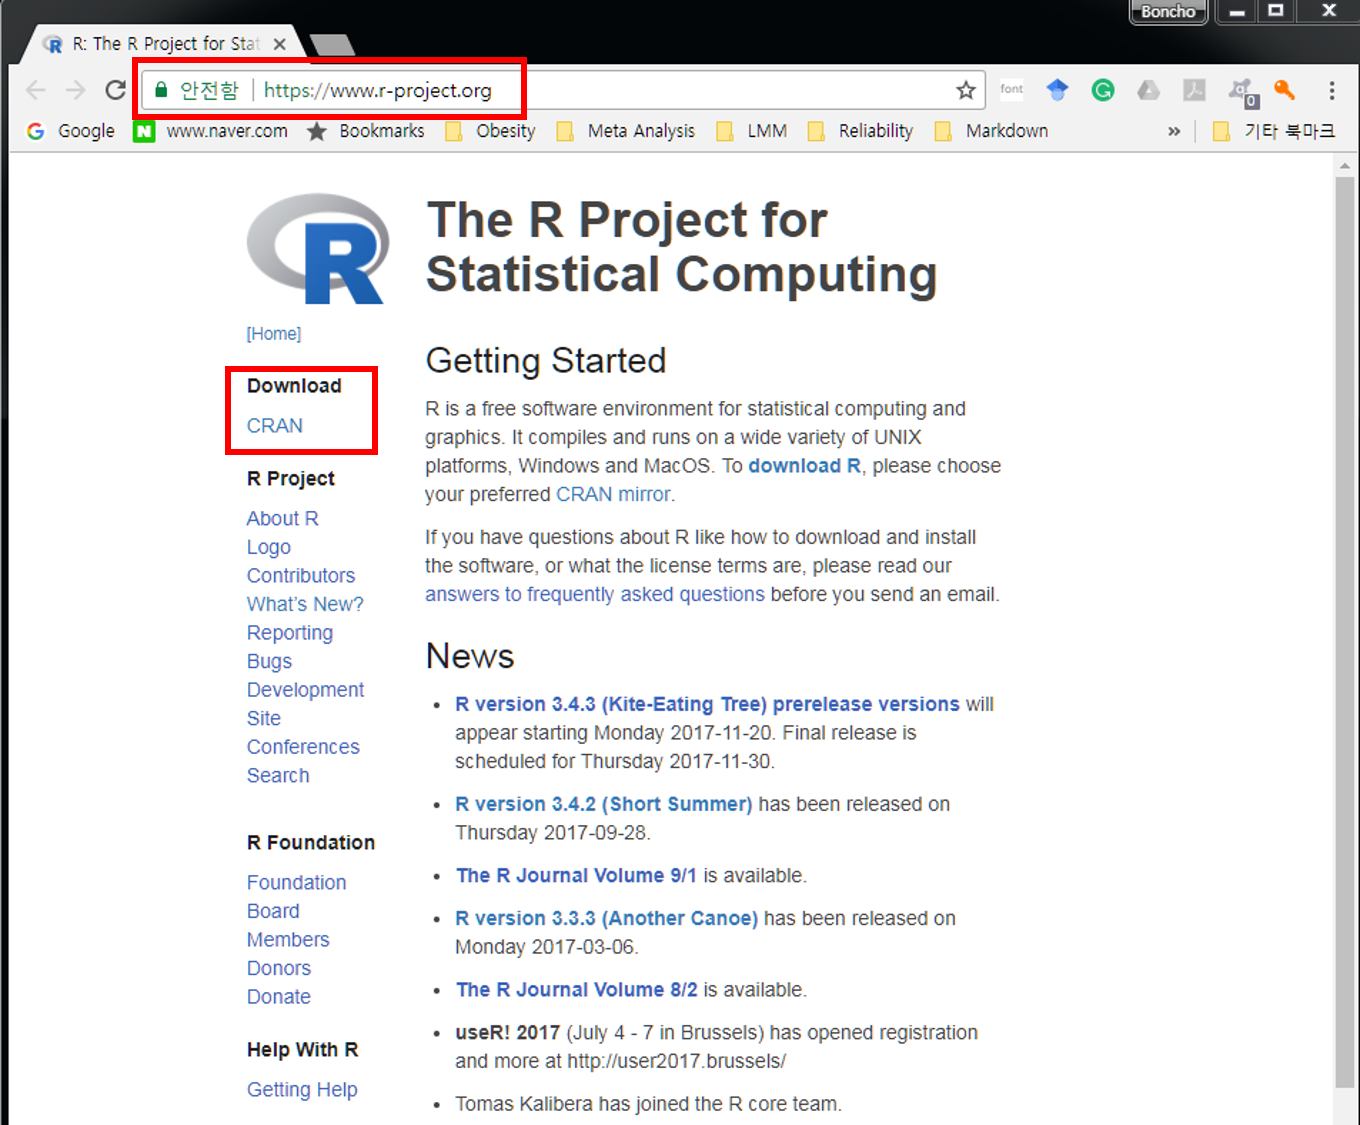
\includegraphics[width=0.9\linewidth]{figures/Rorg-main-add} \end{center}

\normalsize

\begin{enumerate}
\def\labelenumi{\arabic{enumi}.}
\setcounter{enumi}{2}
\tightlist
\item
  클릭 후 연결한 페이지를 스크롤 후 Korea 아래 링크\footnote{해당 링크들은 접속 시점에 따라 변경될 수 있음} 클릭
\end{enumerate}

\footnotesize

\begin{center}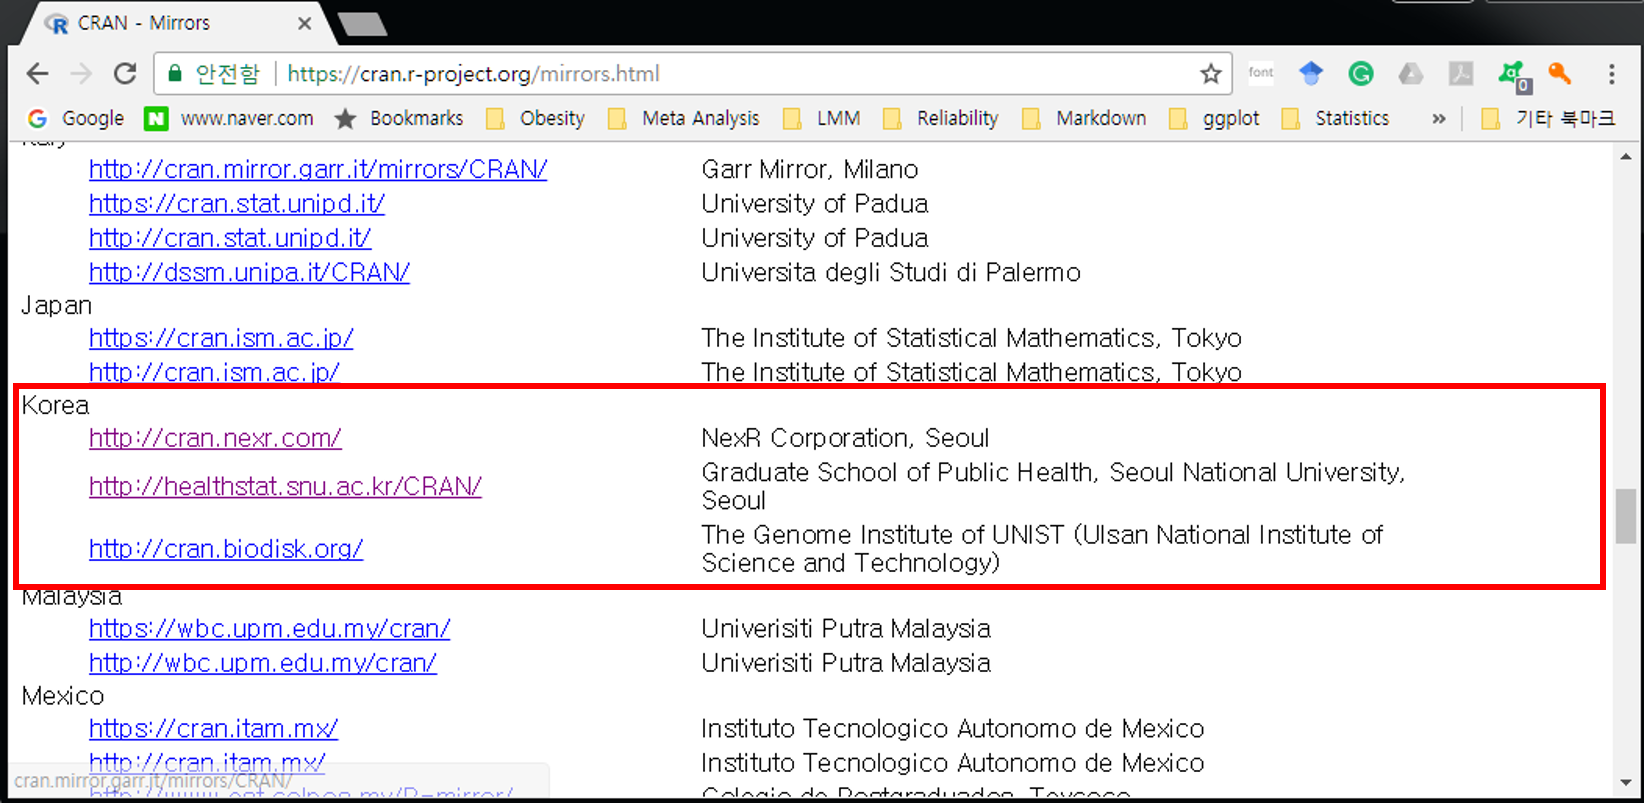
\includegraphics[width=0.9\linewidth]{figures/CRAN-korea-01} \end{center}

\normalsize

\begin{enumerate}
\def\labelenumi{\arabic{enumi}.}
\setcounter{enumi}{3}
\tightlist
\item
  클릭 후 세 가지 운영체제(Linux, Mac OS X, Windowns)에 따른 R 버전 선택 가능\footnote{본 노트는 Windows 버전 설치만 다룸}
\end{enumerate}

\footnotesize

\begin{center}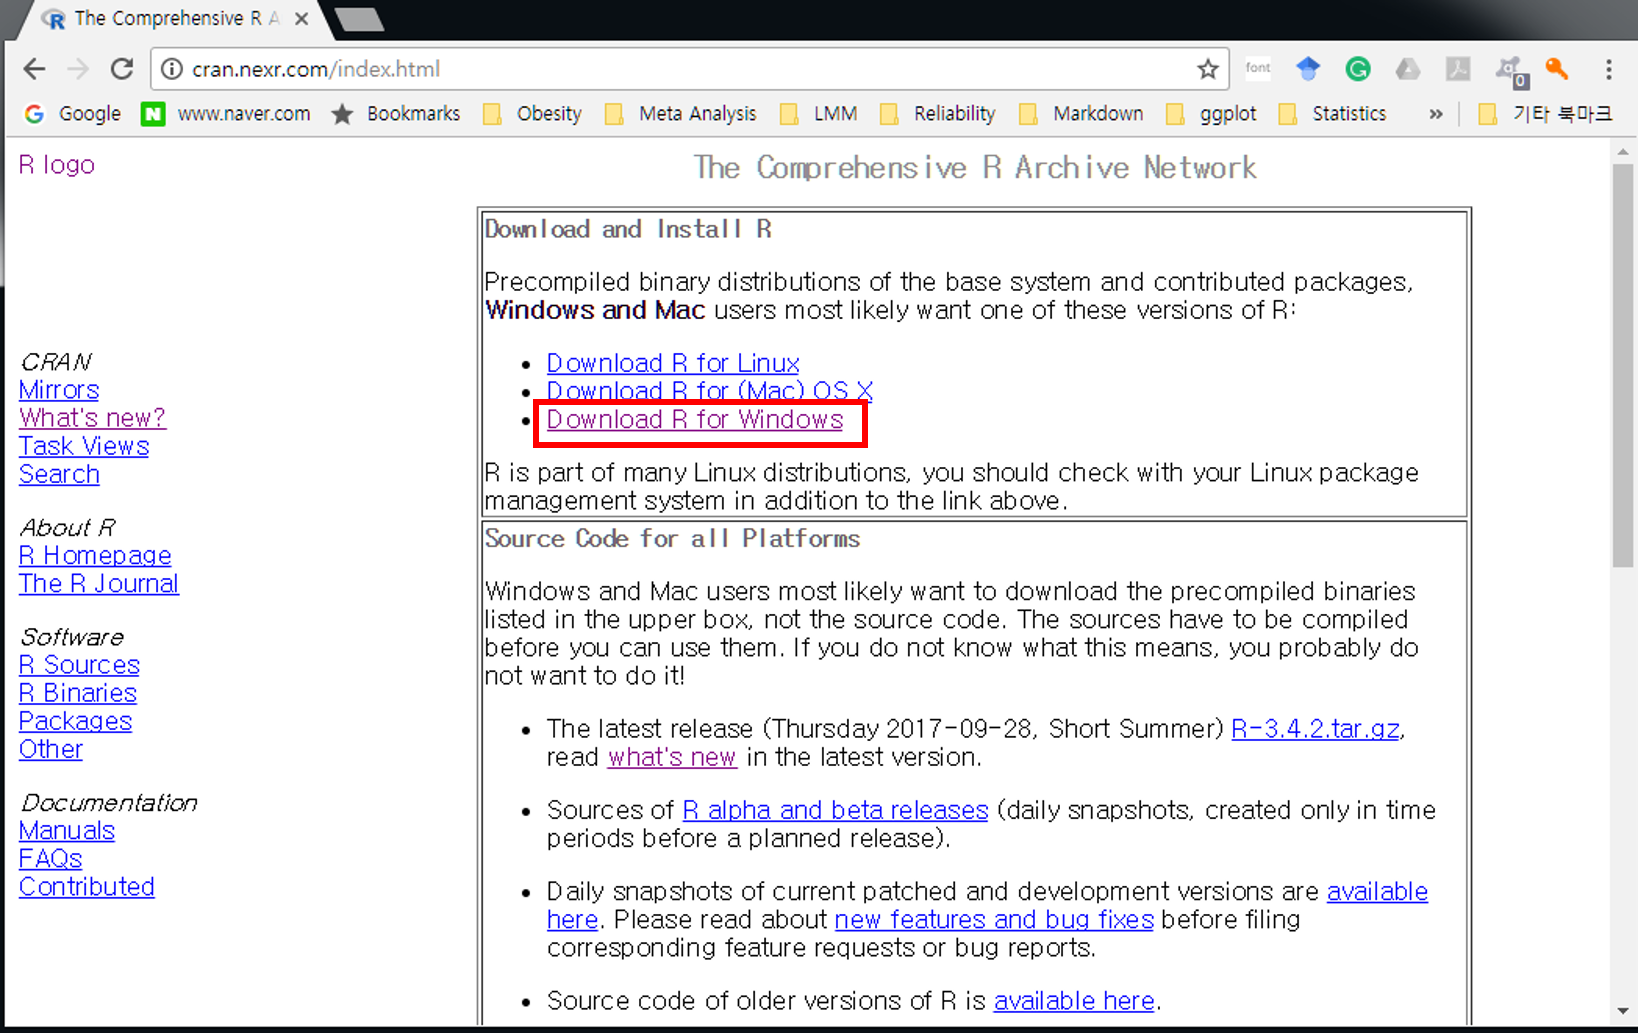
\includegraphics[width=0.9\linewidth]{figures/Rinstall-01} \end{center}

\normalsize

\begin{enumerate}
\def\labelenumi{\arabic{enumi}.}
\setcounter{enumi}{4}
\tightlist
\item
  \textbf{Downloads R for Windows} 링크 클릭하면 다음과 같은 화면으로 이동
\end{enumerate}

\footnotesize

\begin{center}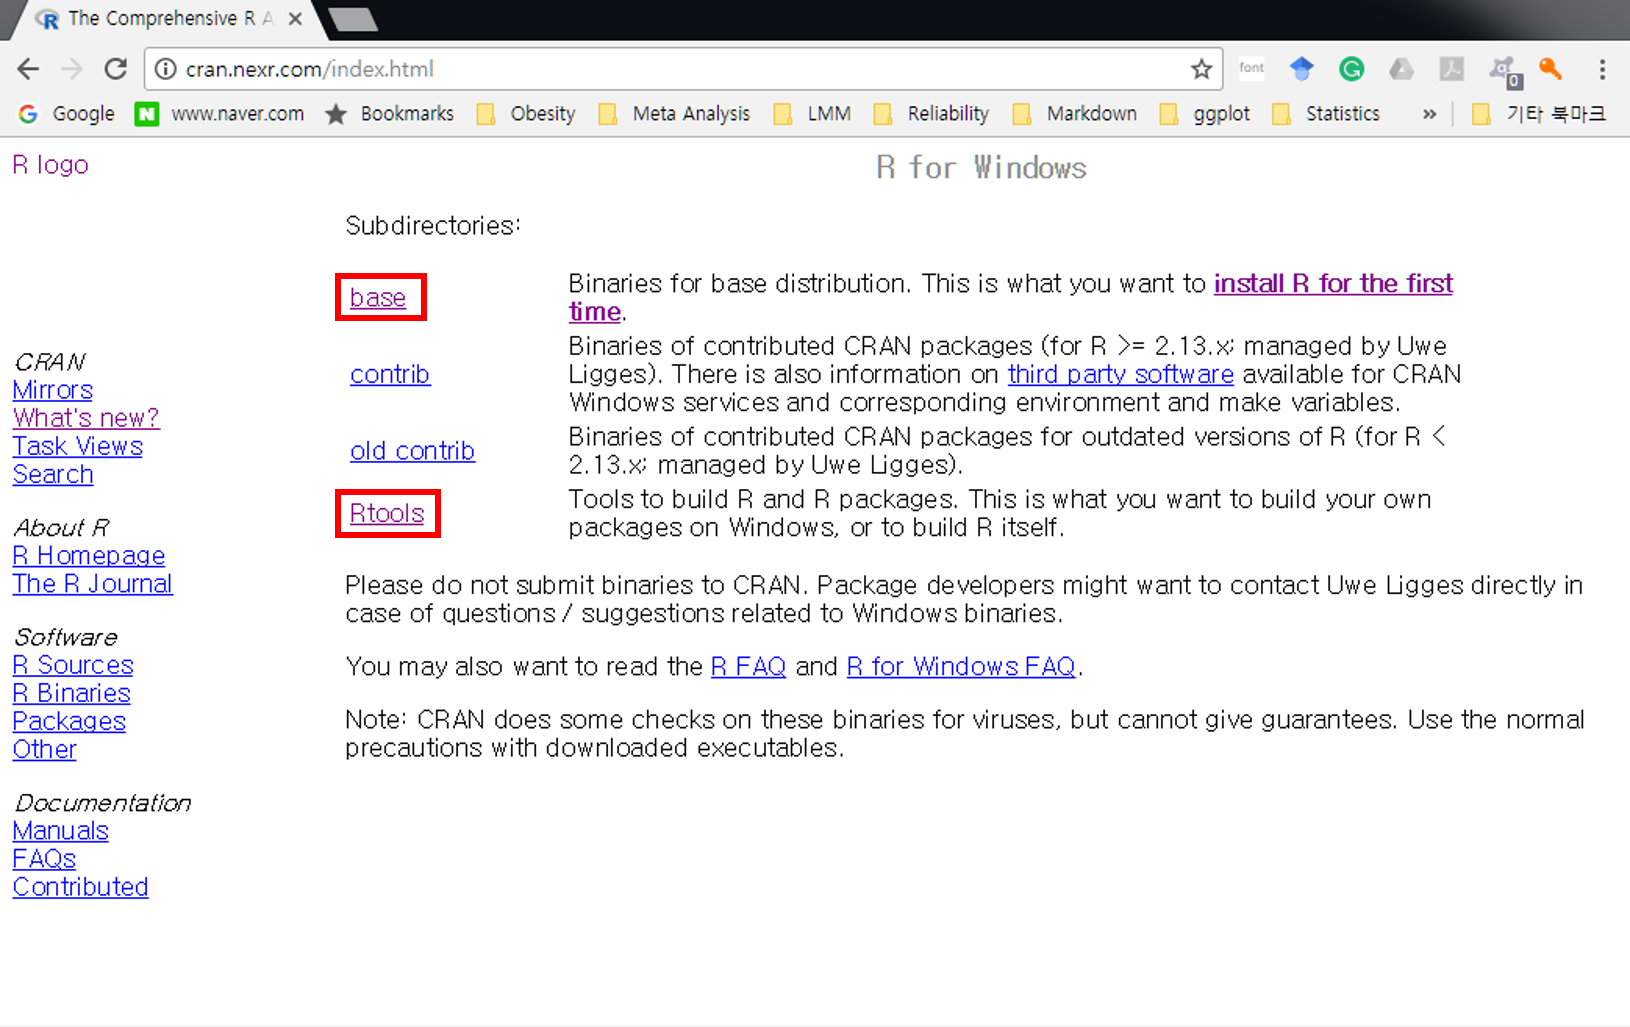
\includegraphics[width=0.9\linewidth]{figures/Rinstall-02} \end{center}

\normalsize

\footnotesize

\BeginKnitrBlock{rmdtip}
다음 하위폴더에 대한 간략 설멍

\begin{itemize}
\tightlist
\item
  \textbf{\texttt{base}}: R 실행 프로그램
\item
  \textbf{\texttt{contrib}}: R package의 바이너리 파일
\item
  \textbf{\texttt{Rtools}}: R package 개발 및 배포를 위한 프로그램
\end{itemize}
\EndKnitrBlock{rmdtip}

\normalsize

\begin{enumerate}
\def\labelenumi{\arabic{enumi}.}
\setcounter{enumi}{5}
\tightlist
\item
  위 화면에서 \textbf{base} 링크 클릭 후 아래 화면에서 \textbf{Downloads R 3.x.x for Windows} 를 클릭 후 설치 파일을 임의의 디렉토리에 저장 및 실행
\end{enumerate}

\footnotesize

\begin{center}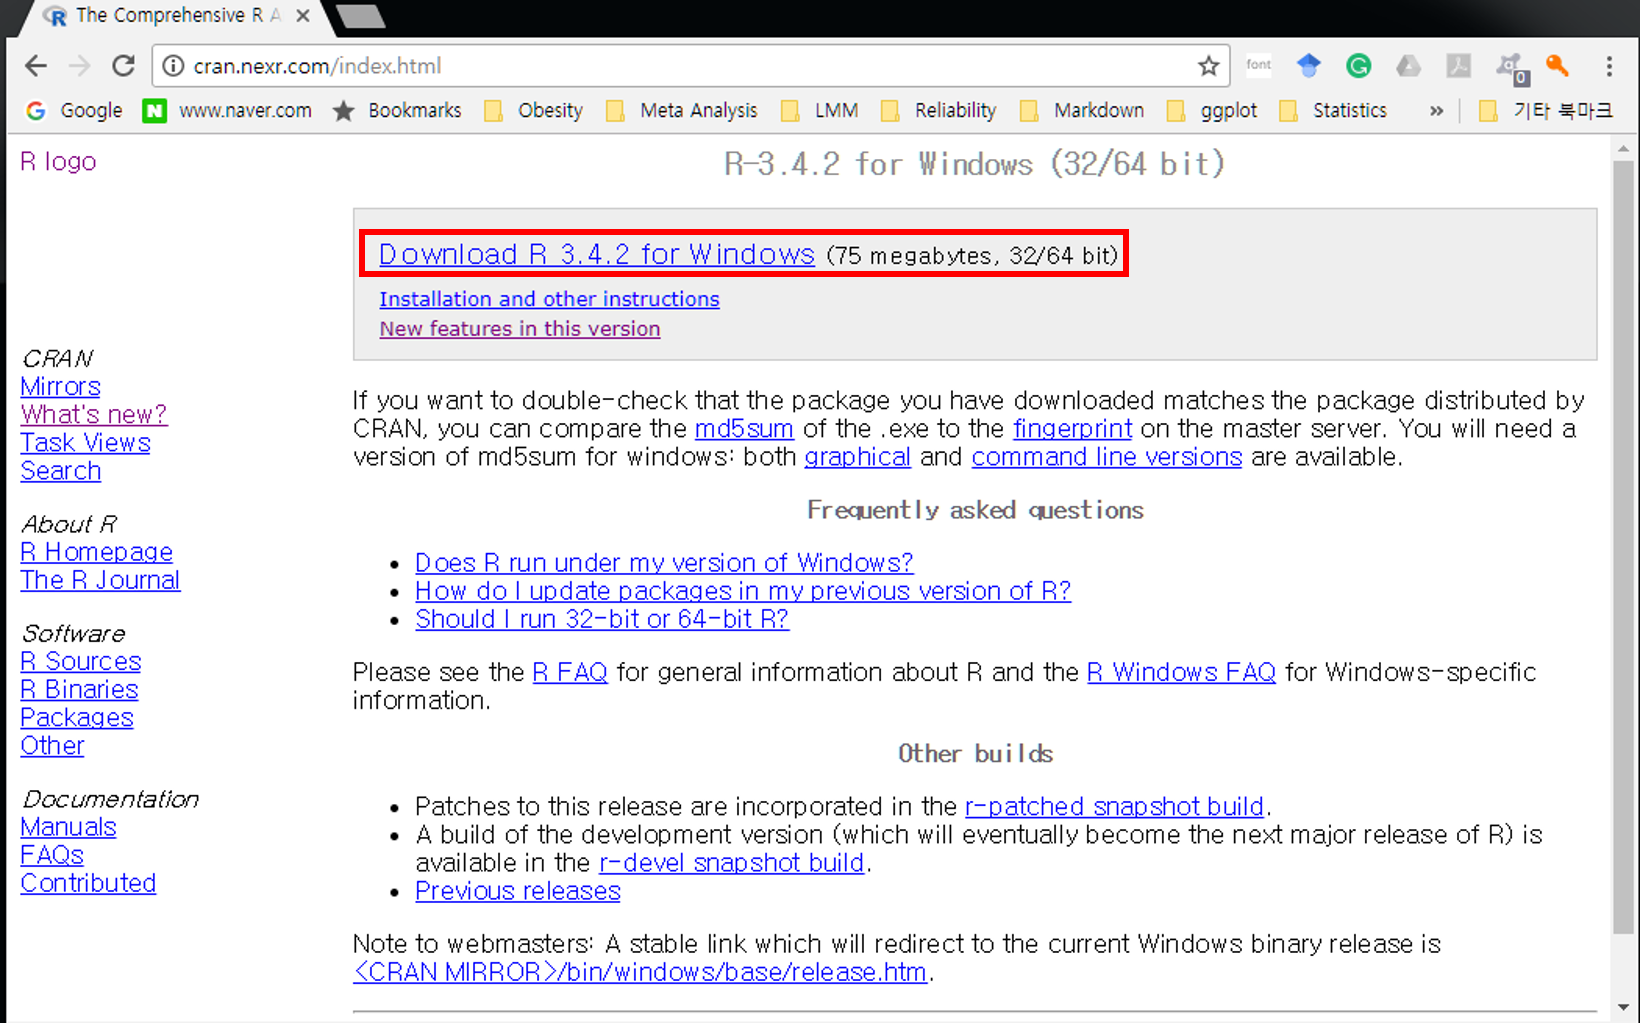
\includegraphics[width=0.9\linewidth]{figures/Rinstall-03} \end{center}

\normalsize

\begin{enumerate}
\def\labelenumi{\arabic{enumi}.}
\setcounter{enumi}{6}
\tightlist
\item
  다운로드한 파일을 실행하면 아래와 같은 대화창이 나타남

  \begin{itemize}
  \tightlist
  \item
    한국어 선택 \(\rightarrow\) 환영 화면에서 {[}다음(N)\textgreater{]} 클릭
  \end{itemize}
\end{enumerate}

\footnotesize

\begin{center}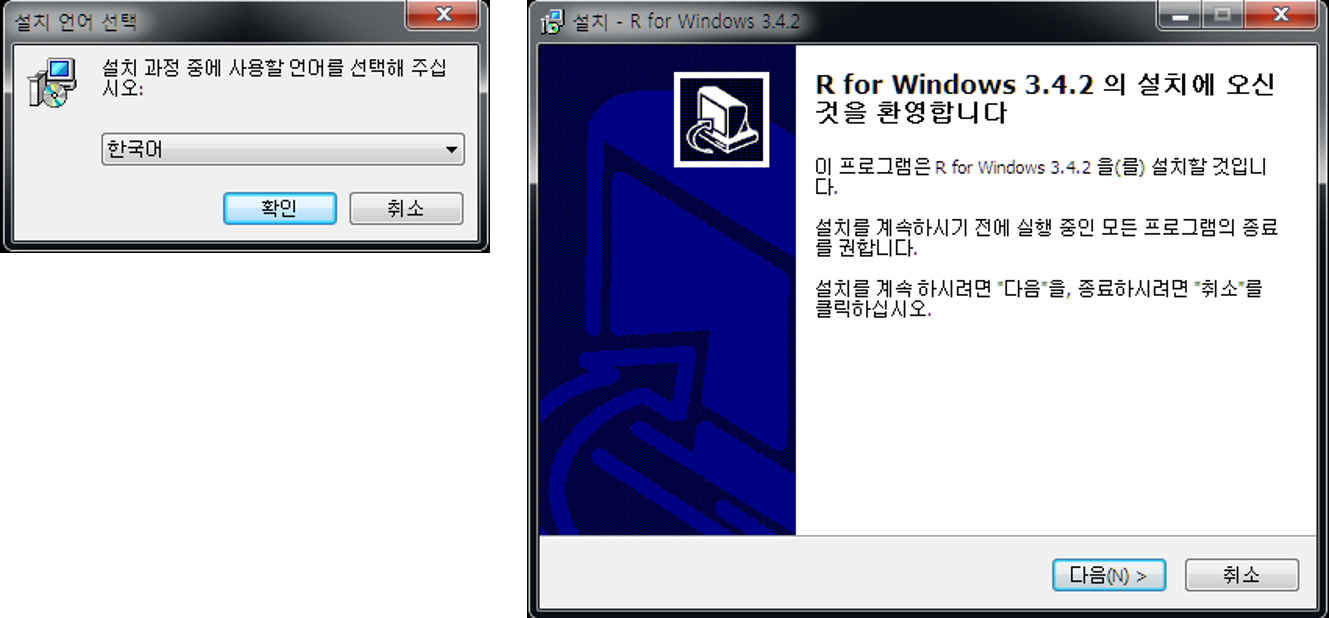
\includegraphics[width=0.9\linewidth]{figures/R-install-F01} \end{center}

\normalsize

\begin{enumerate}
\def\labelenumi{\arabic{enumi}.}
\setcounter{enumi}{7}
\tightlist
\item
  GNU 라이센스에 대한 설명 및 동의 여부({[}다음(N)\textgreater{]}) 클릭
\end{enumerate}

\footnotesize

\begin{center}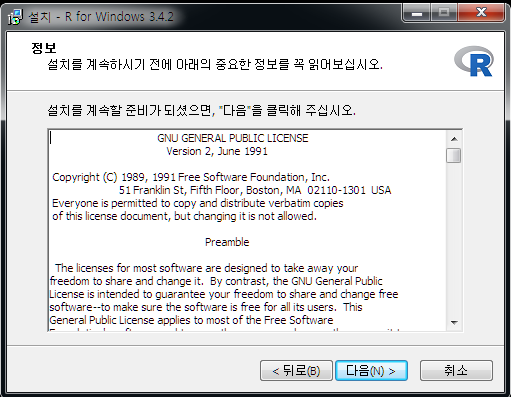
\includegraphics[width=0.9\linewidth]{figures/R-install-F02} \end{center}

\normalsize

\begin{enumerate}
\def\labelenumi{\arabic{enumi}.}
\setcounter{enumi}{8}
\tightlist
\item
  설치 디렉토리 설정 및 구성요소 설지 여부

  \begin{itemize}
  \tightlist
  \item
    원하는 디렉토리 설정(예: \texttt{C:\textbackslash{}R\textbackslash{}R-3.x.x})
  \item
    기본 프로그램(``Core Files''), 32 또는 64 bit 용 설치 파일, R console 한글 번역 모두 체크 뒤 {[}다음(N)\textgreater{]} 클릭
  \end{itemize}
\end{enumerate}

\footnotesize

\begin{center}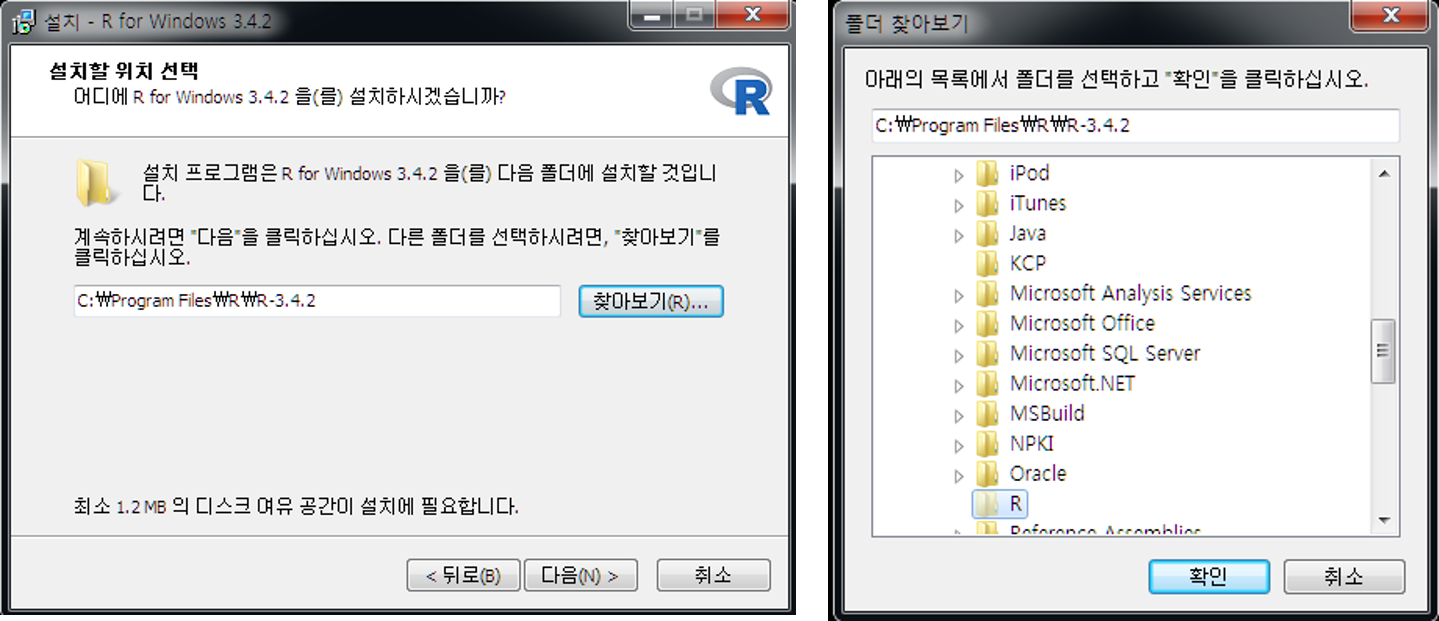
\includegraphics[width=0.9\linewidth]{figures/R-install-F03} \end{center}

\normalsize

\footnotesize

\begin{center}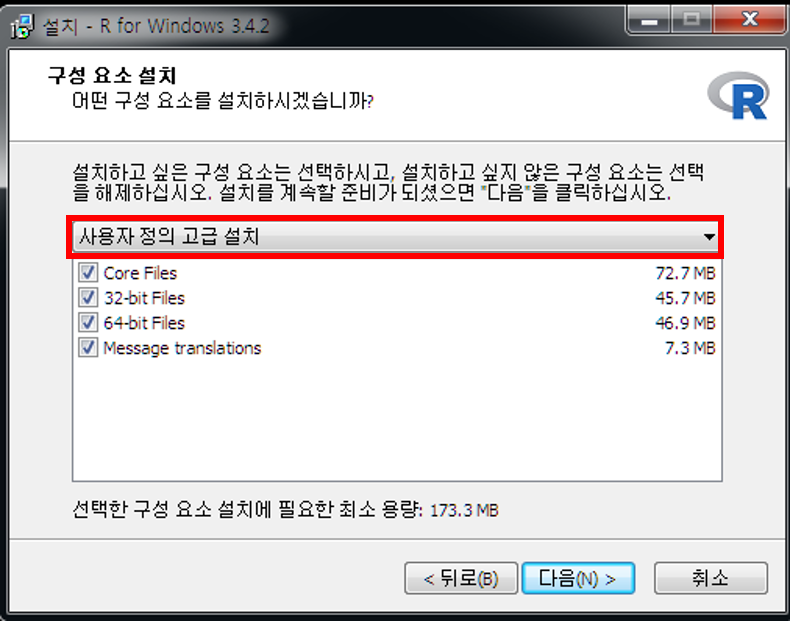
\includegraphics[width=0.9\linewidth]{figures/R-install-F04} \end{center}

\normalsize

\begin{enumerate}
\def\labelenumi{\arabic{enumi}.}
\setcounter{enumi}{9}
\tightlist
\item
  R 스타트업 옵션 지정
\end{enumerate}

\begin{itemize}
\tightlist
\item
  기본값(``No'' check-button)으로도 설치 진행 가능
\item
  본 문서에서는 스타트업 옵션 변경으로 진행
\end{itemize}

\footnotesize

\begin{center}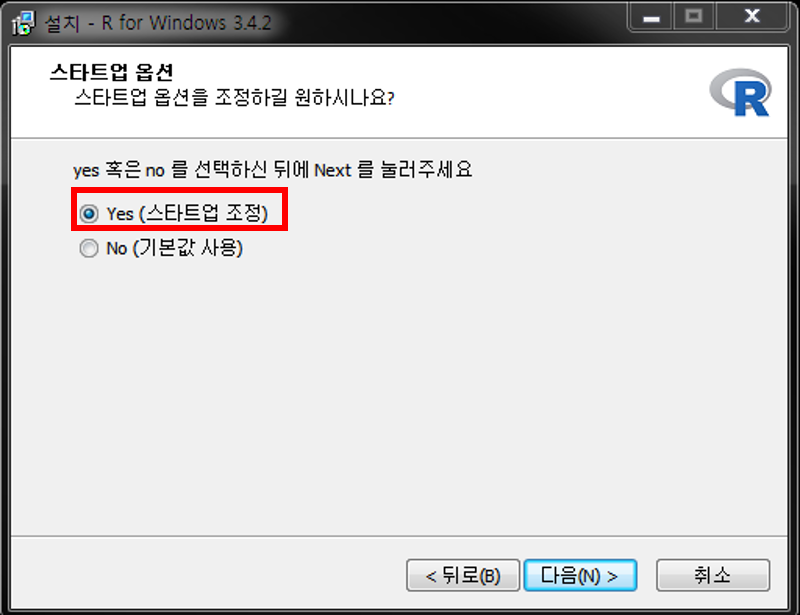
\includegraphics[width=0.9\linewidth]{figures/R-install-F05} \end{center}

\normalsize

\begin{enumerate}
\def\labelenumi{\arabic{enumi}.}
\setcounter{enumi}{10}
\tightlist
\item
  화면표시방식(디스플레이 모드) 설정 변경
\end{enumerate}

\begin{itemize}
\tightlist
\item
  MDI: 한 윈도우 내에서 script 편집창, 출력, 도움말 창 사용
\item
  SDI: 다중 창에서 각각 script 편집창, 출력, 도움말 등을 독립적으로 열기
\end{itemize}

\footnotesize

\begin{center}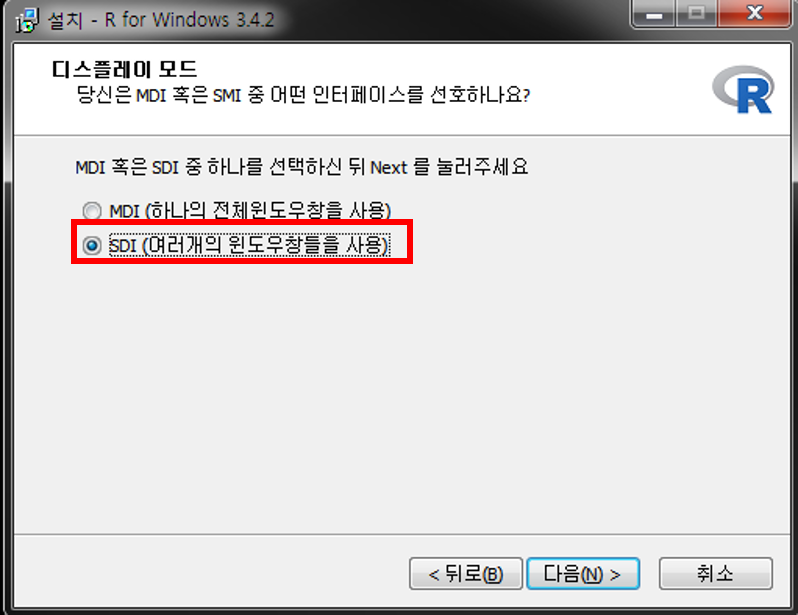
\includegraphics[width=0.9\linewidth]{figures/R-install-F06} \end{center}

\normalsize

\begin{enumerate}
\def\labelenumi{\arabic{enumi}.}
\setcounter{enumi}{11}
\tightlist
\item
  도움말 형식에서 HTML 도움말 기반 선택
\end{enumerate}

\footnotesize

\begin{center}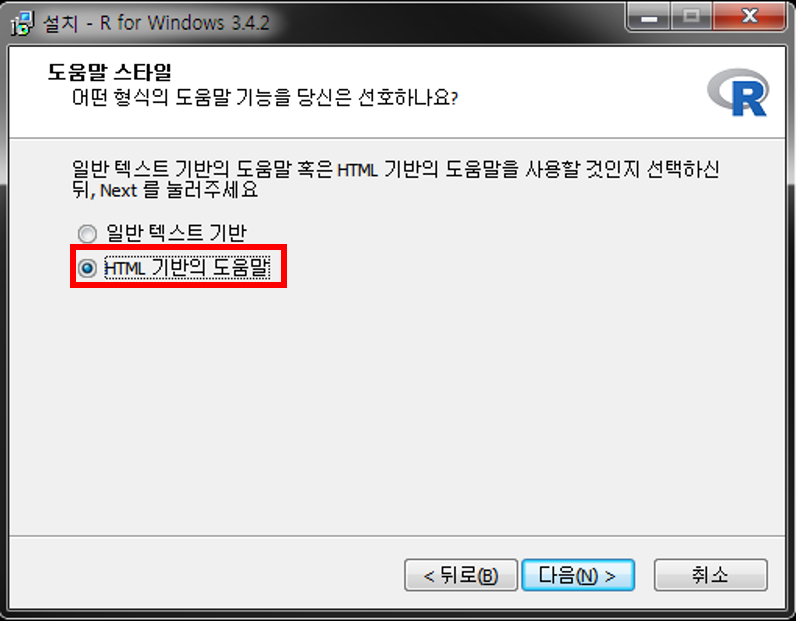
\includegraphics[width=0.9\linewidth]{figures/R-install-F07} \end{center}

\normalsize

\begin{enumerate}
\def\labelenumi{\arabic{enumi}.}
\setcounter{enumi}{12}
\tightlist
\item
  시작메뉴 폴더 선택
\end{enumerate}

\begin{itemize}
\tightlist
\item
  ``바로가기''를 생성할 시작 메뉴 폴더 지정 후 {[}다음(N)\textgreater{]} 클릭 후 설치 진행
\item
  하단 ``시작메뉴 폴더 만들지 않음'' 체크박스 표시 시 시작메뉴에 ``바로가기'' 아이콘이 생성되지 않음(실행에 전혀 지장 없음)
\end{itemize}

\footnotesize

\begin{center}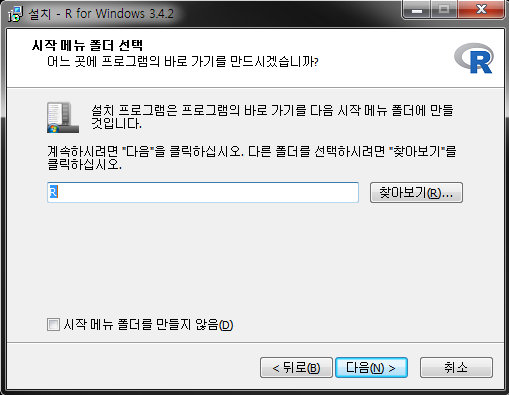
\includegraphics[width=0.9\linewidth]{figures/R-install-F08} \end{center}

\normalsize

\begin{enumerate}
\def\labelenumi{\arabic{enumi}.}
\setcounter{enumi}{13}
\tightlist
\item
  추가 옵션 지정: 바탕화면 아이콘 생성 등 추가적 작업 옵션 체크 후 {[}다음(N)\textgreater{]} 클릭 \(\rightarrow\) 설치 진행
\end{enumerate}

\begin{itemize}
\tightlist
\item
  설치된 R 버전 정보 레지스트리 저장 여부
\item
  \texttt{.Rdata} 확장자를 R 실행파일과 자동 연계
\end{itemize}

\footnotesize

\begin{center}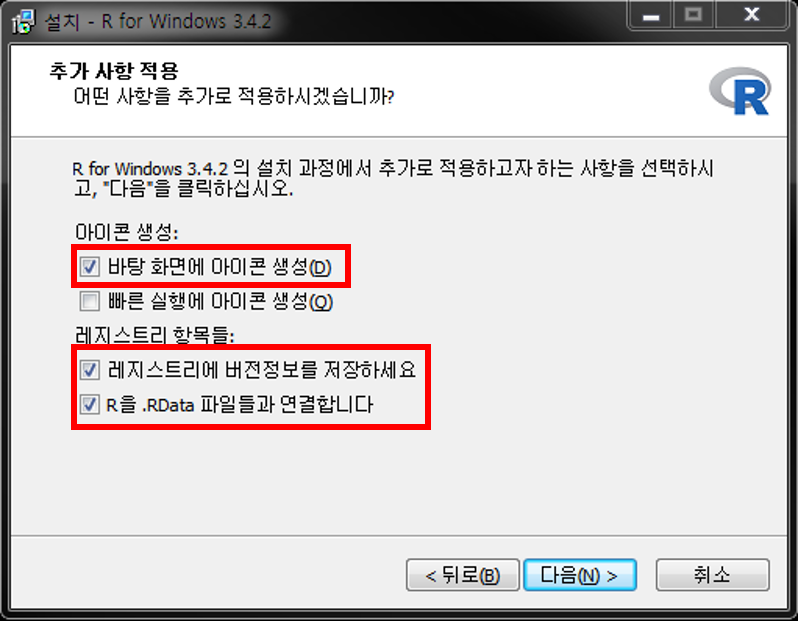
\includegraphics[width=0.9\linewidth]{figures/R-install-F09} \end{center}

\normalsize

\begin{enumerate}
\def\labelenumi{\arabic{enumi}.}
\setcounter{enumi}{14}
\tightlist
\item
  설치 완료 후 바탕화면의 R 아이콘을 더블클릭하면 Rgui가 실행
\end{enumerate}

\footnotesize

\begin{figure}

{\centering 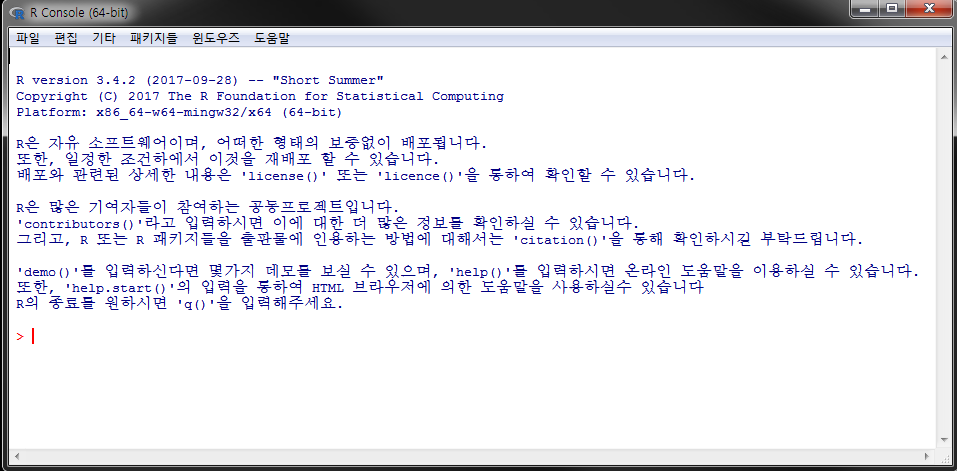
\includegraphics[width=1\linewidth]{figures/Rgui} 

}

\caption{Windows에서 R 실행화면(콘솔 창, SDI 모드)}\label{fig:r-console}
\end{figure}

\normalsize

\hypertarget{r-check}{%
\section{R 시작 및 작동 체크}\label{r-check}}

\BeginKnitrBlock{rmdimportant}
\textbf{실습}: 설치된 R을 실행 후 보이는 R 콘솔(consle) 창에서 명령어를 실행하고 결과 확인
\EndKnitrBlock{rmdimportant}

Figure \ref{fig:r-console} 에서 \texttt{\textgreater{}} 기호는 R의 명령 프롬프트(prompt) 임

\begin{enumerate}
\def\labelenumi{\arabic{enumi}.}
\tightlist
\item
  현재 R session 정보(R 설치 버전, locale, 로딩 packages) 출력
\end{enumerate}

\footnotesize

\begin{Shaded}
\begin{Highlighting}[]
\CommentTok{# R의 설치 버전 및 현재 설정된 locale(언어, 시간대) 및 로딩된 R package 정보 출력}
\KeywordTok{sessionInfo}\NormalTok{() }
\end{Highlighting}
\end{Shaded}

\begin{verbatim}
R version 3.6.2 (2019-12-12)
Platform: x86_64-w64-mingw32/x64 (64-bit)
Running under: Windows 10 x64 (build 18363)

Matrix products: default

locale:
[1] LC_COLLATE=Korean_Korea.949  LC_CTYPE=Korean_Korea.949   
[3] LC_MONETARY=Korean_Korea.949 LC_NUMERIC=C                
[5] LC_TIME=Korean_Korea.949    

attached base packages:
[1] stats     graphics  grDevices utils     datasets  methods   base     

loaded via a namespace (and not attached):
 [1] compiler_3.6.2  magrittr_1.5    bookdown_0.16   tools_3.6.2    
 [5] htmltools_0.4.0 yaml_2.2.1      Rcpp_1.0.3      stringi_1.4.5  
 [9] rmarkdown_2.1   knitr_1.28      stringr_1.4.0   xfun_0.12      
[13] digest_0.6.23   rlang_0.4.4     evaluate_0.14  
\end{verbatim}

\normalsize

\begin{enumerate}
\def\labelenumi{\arabic{enumi}.}
\setcounter{enumi}{1}
\tightlist
\item
  문자열 출력
\end{enumerate}

\footnotesize

\begin{Shaded}
\begin{Highlighting}[]
\CommentTok{#문자열 출력}
\KeywordTok{print}\NormalTok{(}\StringTok{"Hello R"}\NormalTok{) }\CommentTok{#문자열}
\end{Highlighting}
\end{Shaded}

\begin{verbatim}
[1] "Hello R"
\end{verbatim}

\normalsize

\begin{quote}
\texttt{\#} 기호는 주석의 시작을 의미하고 실제로 실행되지 않음 같은 행에서 \texttt{\#} 뒤 내용의 코드 역시 실행되지 않음
\end{quote}

\begin{enumerate}
\def\labelenumi{\arabic{enumi}.}
\setcounter{enumi}{2}
\tightlist
\item
  \texttt{a} 라는 변수에 숫자 9, \texttt{b}라는 변수에 숫자 7를 할당 후 출력
\end{enumerate}

\footnotesize

\begin{Shaded}
\begin{Highlighting}[]
\CommentTok{# 수치형 값(scalar)을 변수에 할당(assign)}
\CommentTok{# 여러 명령어를 한줄에 입력할 때에는 세미콜론(;)으로 구분}
\NormalTok{a =}\StringTok{ }\DecValTok{9}\NormalTok{; b =}\StringTok{ }\DecValTok{7}
\NormalTok{a}
\end{Highlighting}
\end{Shaded}

\begin{verbatim}
[1] 9
\end{verbatim}

\begin{Shaded}
\begin{Highlighting}[]
\NormalTok{b}
\end{Highlighting}
\end{Shaded}

\begin{verbatim}
[1] 7
\end{verbatim}

\normalsize

\begin{enumerate}
\def\labelenumi{\arabic{enumi}.}
\setcounter{enumi}{3}
\tightlist
\item
  변수 \texttt{a}와 \texttt{b}의 사칙연산
\end{enumerate}

\footnotesize

\begin{Shaded}
\begin{Highlighting}[]
\NormalTok{a}\OperatorTok{+}\NormalTok{b; a}\OperatorTok{-}\NormalTok{b; a}\OperatorTok{*}\NormalTok{b; a}\OperatorTok{/}\NormalTok{b}
\end{Highlighting}
\end{Shaded}

\begin{verbatim}
[1] 16
\end{verbatim}

\begin{verbatim}
[1] 2
\end{verbatim}

\begin{verbatim}
[1] 63
\end{verbatim}

\begin{verbatim}
[1] 1.285714
\end{verbatim}

\normalsize

\begin{enumerate}
\def\labelenumi{\arabic{enumi}.}
\setcounter{enumi}{4}
\tightlist
\item
  R 그래픽 맛보기: 정규분포로부터 난수 100개 생성 후 생성된 데이터에 대한 히스토그램 작성
\end{enumerate}

\footnotesize

\begin{Shaded}
\begin{Highlighting}[]
\CommentTok{# 난수 생성 시 값은 매번 달라지기 때문에 seed를 주어 일정값이 생성되도록 고정}
\CommentTok{# "="과 "<-"는 모두 동일한 기능을 가진 할당 연산자임}
\CommentTok{#평균이 0 이고 분산이 1인 정규분포에서 난수 100개 생성}
\KeywordTok{set.seed}\NormalTok{(}\DecValTok{12345}\NormalTok{) }\CommentTok{# random seed 지정}
\NormalTok{x <-}\StringTok{ }\KeywordTok{rnorm}\NormalTok{(}\DecValTok{100}\NormalTok{) }\CommentTok{# 난수 생성}
\KeywordTok{hist}\NormalTok{(x) }\CommentTok{# 히스토그램}
\end{Highlighting}
\end{Shaded}

\begin{figure}

{\centering 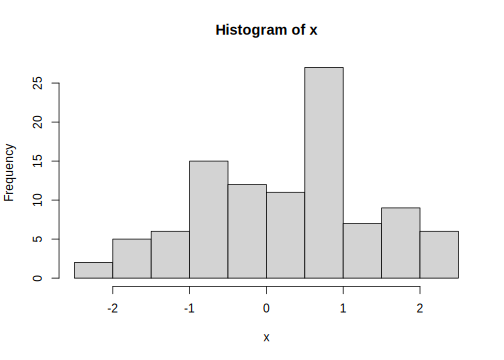
\includegraphics{01-overview_files/figure-latex/check-04-1} 

}

\caption{정규분포 100개의 히스토그램}\label{fig:check-04}
\end{figure}

\normalsize

\footnotesize

\BeginKnitrBlock{rmdtip}
R 명령어 또는 전체 프로그램 소스 실행 시 매우 빈번히 오류가 나타나는데, 이를 해결할 수 있는 가장 좋은 방법은 앞에서 언급한 Google을 이용한 검색 또는 R 설치 시 자체적으로 내장되어 있는 도움말을 참고하는 것이 가장 효율적임.
\EndKnitrBlock{rmdtip}

\normalsize

\footnotesize

\begin{table}[H]

\caption{\label{tab:tab-help}R help 관련 명령어 리스트}
\centering
\fontsize{10}{12}\selectfont
\begin{tabular}[t]{l>{\raggedright\arraybackslash}p{5cm}l}
\toprule
도움말 보기 명령어 & 설명 & 사용법\\
\midrule
\rowcolor{gray!6}  `help` 또는 `?` & 도움말 시스템 호출 & `help(함수명)`\\
`help.search` 또는 `??` & 주어진 문자열을 포함한 문서 검색 & `help.search(pattern)`\\
\rowcolor{gray!6}  `example` & topic의 도움말 페이지에 있는 examples section 실행 & `example(함수명)`\\
`vignette` & topic의 pdf 또는 html 레퍼런스 메뉴얼 불러오기 & `vignette(패키지명 또는 패턴)`\\
\bottomrule
\end{tabular}
\end{table}

\normalsize

\footnotesize

\BeginKnitrBlock{rmdtip}
\textbf{Vignette} 의 활용

\begin{itemize}
\tightlist
\item
  \texttt{vignette()}에서 제공하는 문서는 데이터를 기반으로 사용하고자 하는 패키지의 실제 활용 예시를 작성한 문서이기 때문에 초보자들이 R 패키지 활용에 대한 접근성을 높혀줌.
\item
  \texttt{browseVignettes()} 명령어를 통해 vignette을 제공하는 R 패키지 및 해당 vignette 문서 확인 가능
\end{itemize}
\EndKnitrBlock{rmdtip}

\normalsize

\hypertarget{rconsle-script}{%
\section{R script 편집기 사용}\label{rconsle-script}}

\BeginKnitrBlock{rmdimportant}
\textbf{실습}: R 설치 후 Rgui 에서 제공하는 편집기(R editor)에 명령어를 입력하고 실행
\EndKnitrBlock{rmdimportant}

설치된 R을 실행 후 상단 pull-down 메뉴에서 {[}\textbf{File}{]} \(\rightarrow\) {[}\textbf{새 스크립트}{]}를 선택하면 아래 그림과 같이 편집창(R 인스톨 시 SDI 옵션 기준)이 나타남

\footnotesize

\begin{center}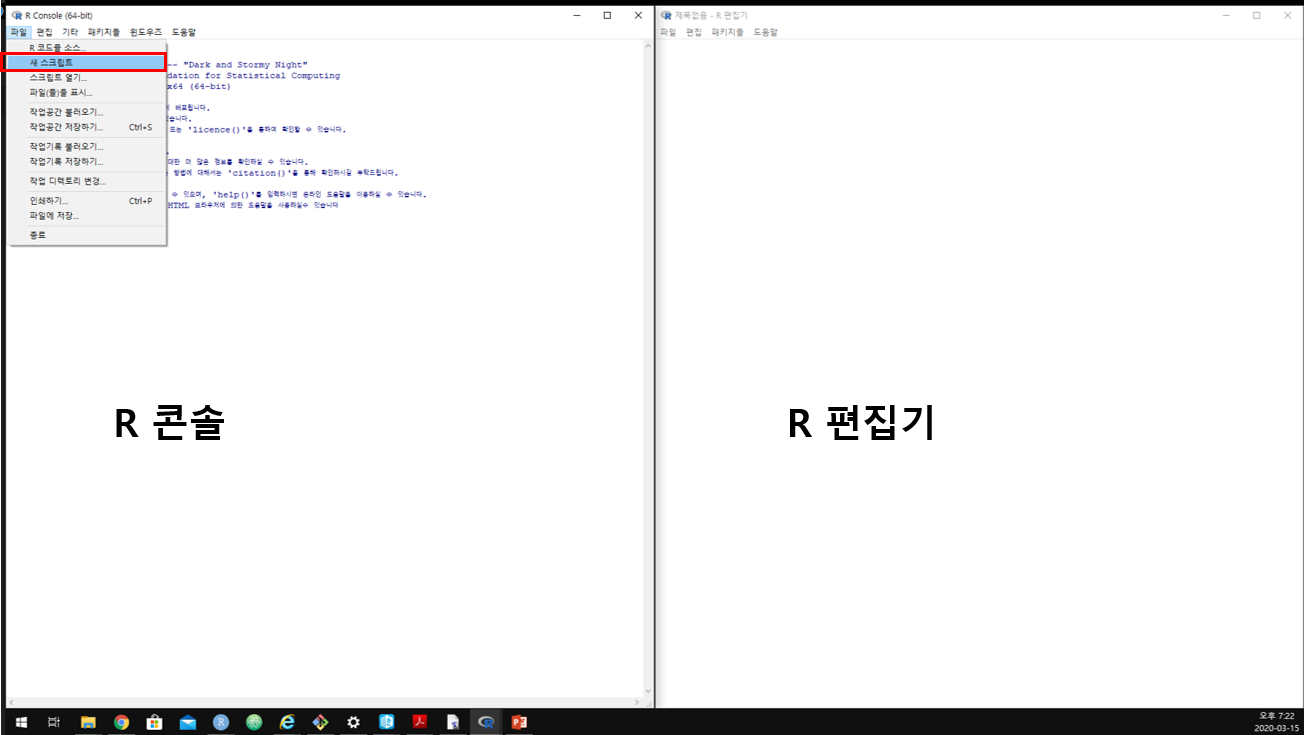
\includegraphics[width=1\linewidth]{figures/r-console-edit} \end{center}

\normalsize

편집기 창에 다음 명령어 입력

\footnotesize

\begin{Shaded}
\begin{Highlighting}[]
\CommentTok{# R에 내장된 cars 데이터셋 불러오기 cars dataset에 포함된 변수들의 기초통계량}
\CommentTok{# 출력 2차원 산점도}
\KeywordTok{data}\NormalTok{(cars)}
\KeywordTok{help}\NormalTok{(cars)  }\CommentTok{# cars 데이터셋에 대한 설명 help 창에 출력}
\KeywordTok{head}\NormalTok{(cars)  }\CommentTok{# cars 데이터셋 처음 6개 행 데이터 출력}
\KeywordTok{summary}\NormalTok{(cars)  }\CommentTok{# cars 데이터셋 요약}
\KeywordTok{plot}\NormalTok{(cars)  }\CommentTok{# 변수가 2개인 경우 산점도 출력}
\end{Highlighting}
\end{Shaded}

\normalsize

\begin{itemize}
\tightlist
\item
  편집창에서 한 줄을 실행시키려면 명령어가 입력된 줄에서 \textbf{{[}Ctrl{]}} + \textbf{{[}R{]}} 입력
\item
  편집창에 입력한 모든 명령어를 실행시키려면 모든 줄을 선택(마우스 또는 {[}Shift{]} + \(\downarrow\))
\end{itemize}

\footnotesize

\begin{verbatim}
  speed dist
1     4    2
2     4   10
3     7    4
4     7   22
5     8   16
6     9   10
\end{verbatim}

\begin{verbatim}
     speed           dist       
 Min.   : 4.0   Min.   :  2.00  
 1st Qu.:12.0   1st Qu.: 26.00  
 Median :15.0   Median : 36.00  
 Mean   :15.4   Mean   : 42.98  
 3rd Qu.:19.0   3rd Qu.: 56.00  
 Max.   :25.0   Max.   :120.00  
\end{verbatim}

\begin{figure}
\centering
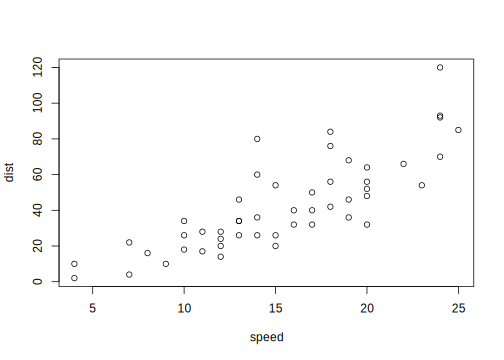
\includegraphics{01-overview_files/figure-latex/check-edit-out-1.pdf}
\caption{\label{fig:check-edit-out}cars 데이터셋의 speed와 dist 간 2차원 산점도: speed는 자동차 속도(mph)이고 dist는 해당 속도에서 브레이크를 밟았을 때 멈출 때 까지 걸린 거리(ft)를 나타냄.}
\end{figure}

\normalsize

\begin{itemize}
\tightlist
\item
  R은 명령어를 입력하고 실행결과를 확인하는 대화형(interpreter) 방식
\item
  콘솔창에서 \(\uparrow\)/\(\downarrow\)를 누르면 이전/이후 실행 명령 기록 확인 가능
\item
  여러 줄 이상 R 명령어라든가 반복적, 장기간 작업을 수행해야 할 경우 R 명령어로 구성된 스크립트 작성 후 일괄 실행하는 것이 일반적
\item
  여러 다중 명령 코딩 시 콘솔창에 직접 입력하는 것은 비효율적이므로 스크립트 에디터를 사용
\item
  위 예시처럼 R 에디터 사용할 수 있으나 가독성 및 코딩 효율이 떨어짐
\item
  과거 많이 사용됐던 R 에디터: \href{http://www.winedt.com}{WinEdt}, \href{https://sourceforge.net/projects/tinn-r/}{Tinn-R}, \href{http://www.vim.org/scripts/script.php?script_id=2628}{Vim}
\item
  현재 가장 범용적 R 에디터: \textbf{Rstudio}
\end{itemize}

\hypertarget{r-studio}{%
\section{RStudio}\label{r-studio}}

\begin{itemize}
\tightlist
\item
  \href{https://rstudio.com/}{RStudio}: R 통합 분석/개발 환경(integrated development environment, IDE)으로 현재 가장 대중적으로 사용되고 있는 R 사용 환경
\item
  명령 곤솔 외 파일 편집, 데이터 객체, 명령 기록(.history), 그래프 등에 쉽게 접근 가능
\item
  RStudio 독자적인 개발 환경 제공: Rmarkdown, Rnotebook, Shiny Web Application 등 다양한 R 환경을 제공
\item
  버전관리(git, subversion)를 통해 project 관리 가능
\item
  \textbf{무료} 및 유료 소프트웨어 제공
\end{itemize}

\hypertarget{rstudio-install}{%
\subsection{RStudio 설치하기}\label{rstudio-install}}

\begin{enumerate}
\def\labelenumi{\arabic{enumi}.}
\tightlist
\item
  웹 브라우저를 통해 \url{https://rstudio.com} 접속 후 상단 \href{https://rstudio.com/products/rstudio/download/}{DOWNLOAD} 링크 클릭
\end{enumerate}

\footnotesize

\begin{center}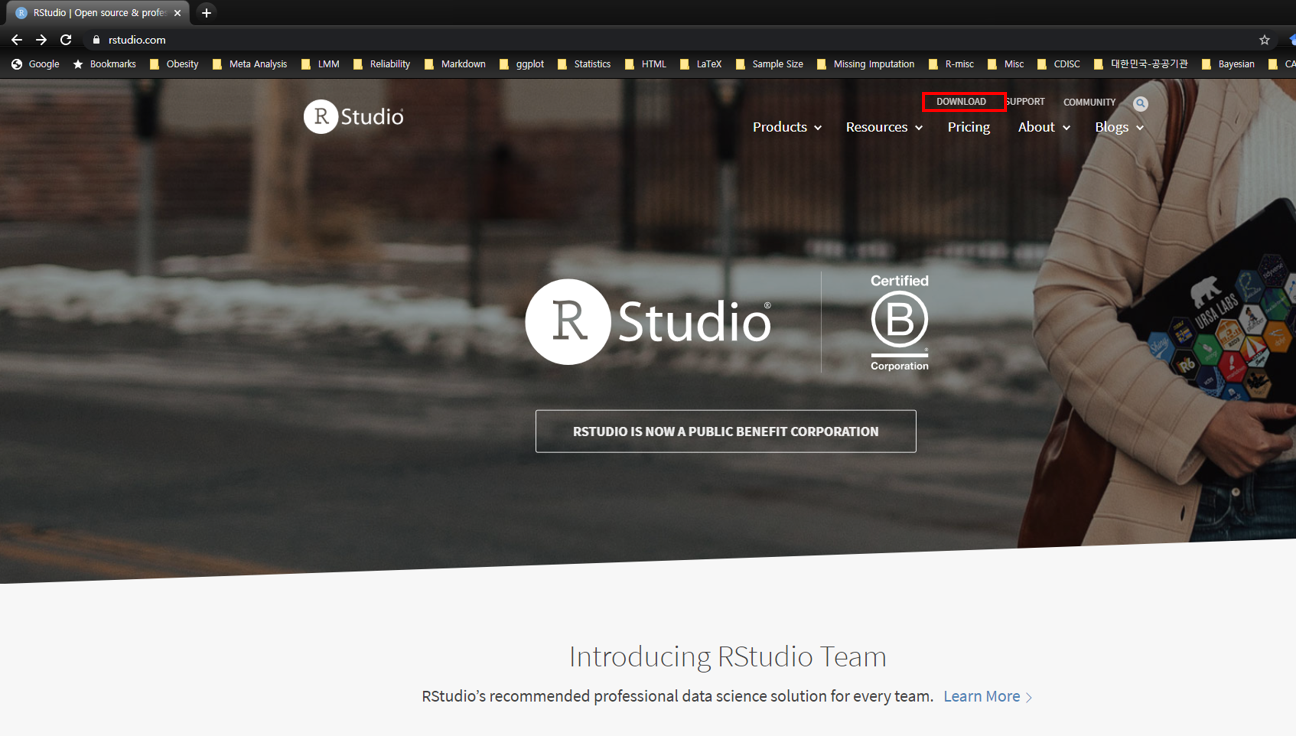
\includegraphics[width=0.8\linewidth]{figures/rstudio-homepage} \end{center}

\normalsize

\begin{enumerate}
\def\labelenumi{\arabic{enumi}.}
\setcounter{enumi}{1}
\item
  Desktop 또는 Server 버전 중 택일

  \begin{itemize}
  \tightlist
  \item
    서버용 설치를 위해서는 Server 클릭 \(\rightarrow\) 소규모 자료 분석용으로는 불필요
  \item
    여기서는 \textbf{Desktop} 버전 선택 후 다음 링크로 이동
  \end{itemize}
\end{enumerate}

\footnotesize

\begin{center}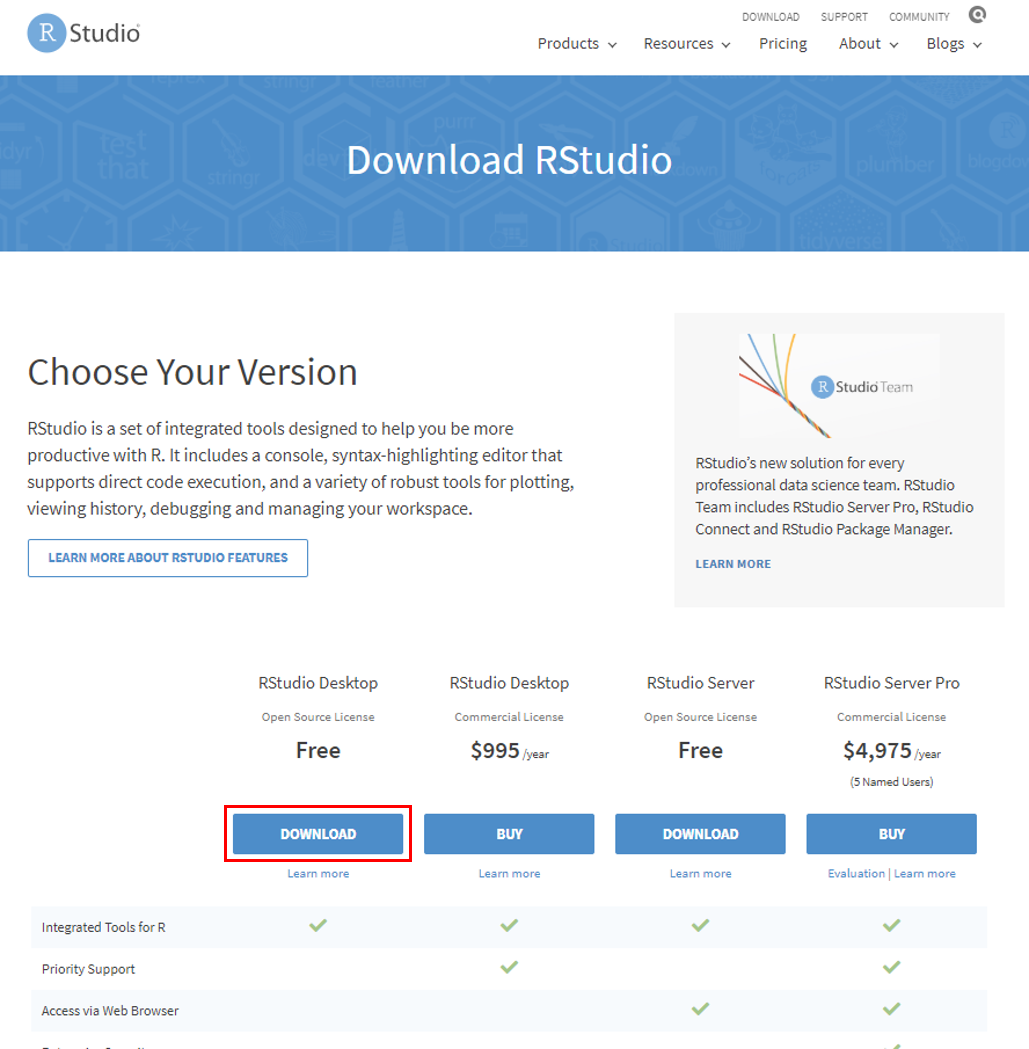
\includegraphics[width=0.7\linewidth]{figures/rstudio-download} \end{center}

\normalsize

\begin{enumerate}
\def\labelenumi{\arabic{enumi}.}
\setcounter{enumi}{2}
\tightlist
\item
  운영체제에 맞는 Rstudio installer 다운로드(여기서는 Windows 버전 다운로드)
\end{enumerate}

\footnotesize

\begin{center}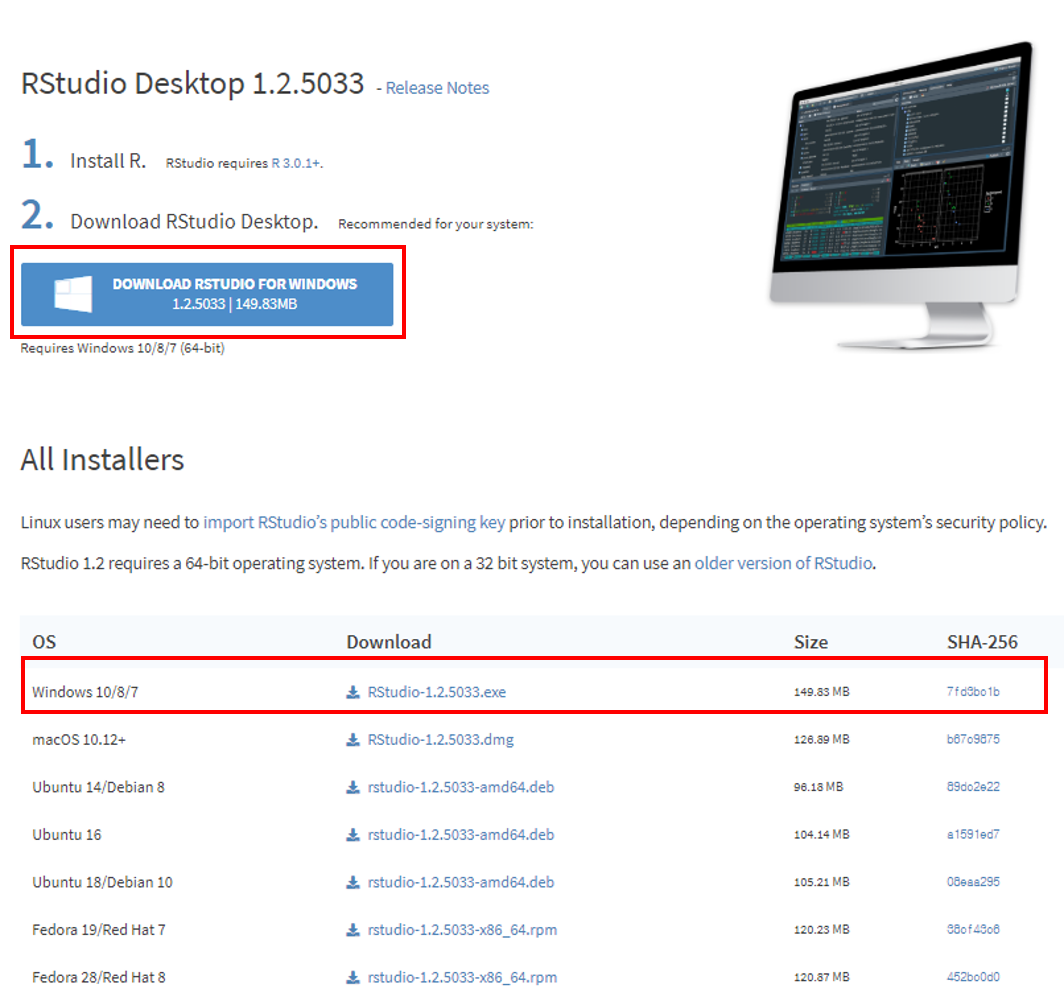
\includegraphics[width=0.6\linewidth]{figures/r-studio-download-02} \end{center}

\normalsize

\begin{enumerate}
\def\labelenumi{\arabic{enumi}.}
\setcounter{enumi}{3}
\tightlist
\item
  RStudio installer 다운로드 시 파일이 저장된 폴더에서 보통 \texttt{RStudio-xx.xx.xxx.exe} 형식의 파일명 확인

  \begin{itemize}
  \tightlist
  \item
    더블 클릭 후 실행
  \item
    \textbf{{[}다음\textgreater{]}} 몇 번 클릭 후 설치 종료
  \end{itemize}
\end{enumerate}

\footnotesize

\begin{center}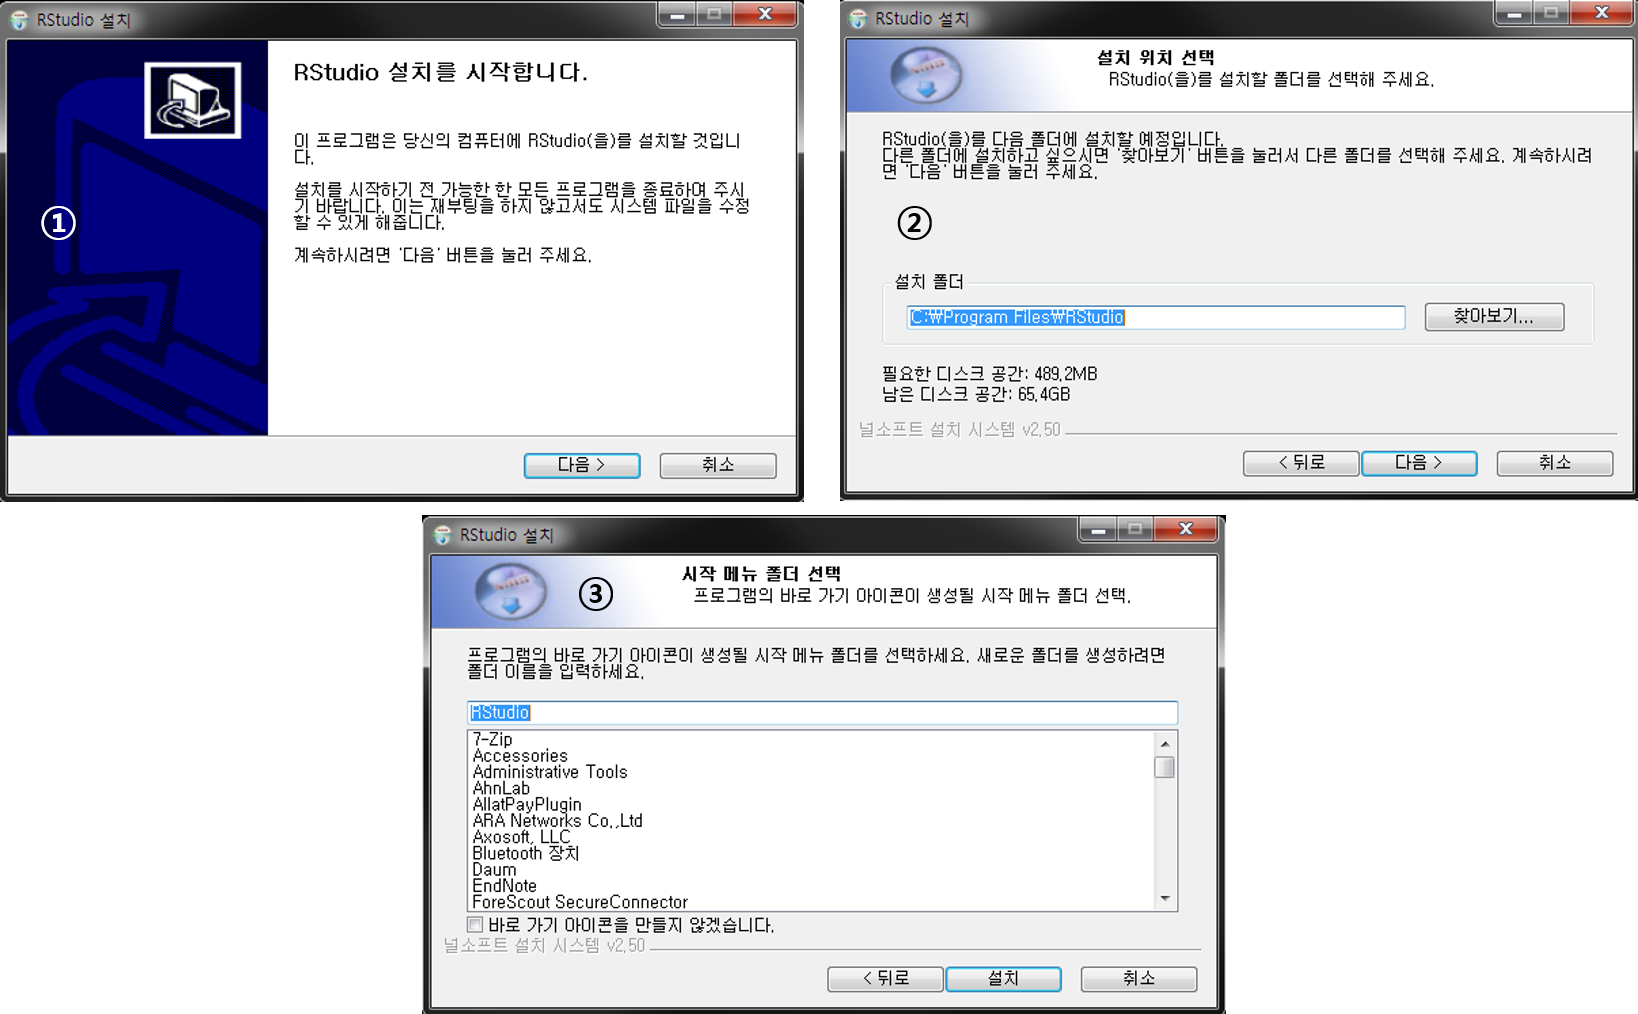
\includegraphics{figures/Rstudio-installer} \end{center}

\normalsize

\begin{enumerate}
\def\labelenumi{\arabic{enumi}.}
\setcounter{enumi}{4}
\tightlist
\item
  바탕화면 혹은 시작 프로그램에 새로 설치된 RStudio 아이콘 클릭 후 아래와 같은 프로그램 창이 나타나면 설치 성공
\end{enumerate}

\footnotesize

\begin{center}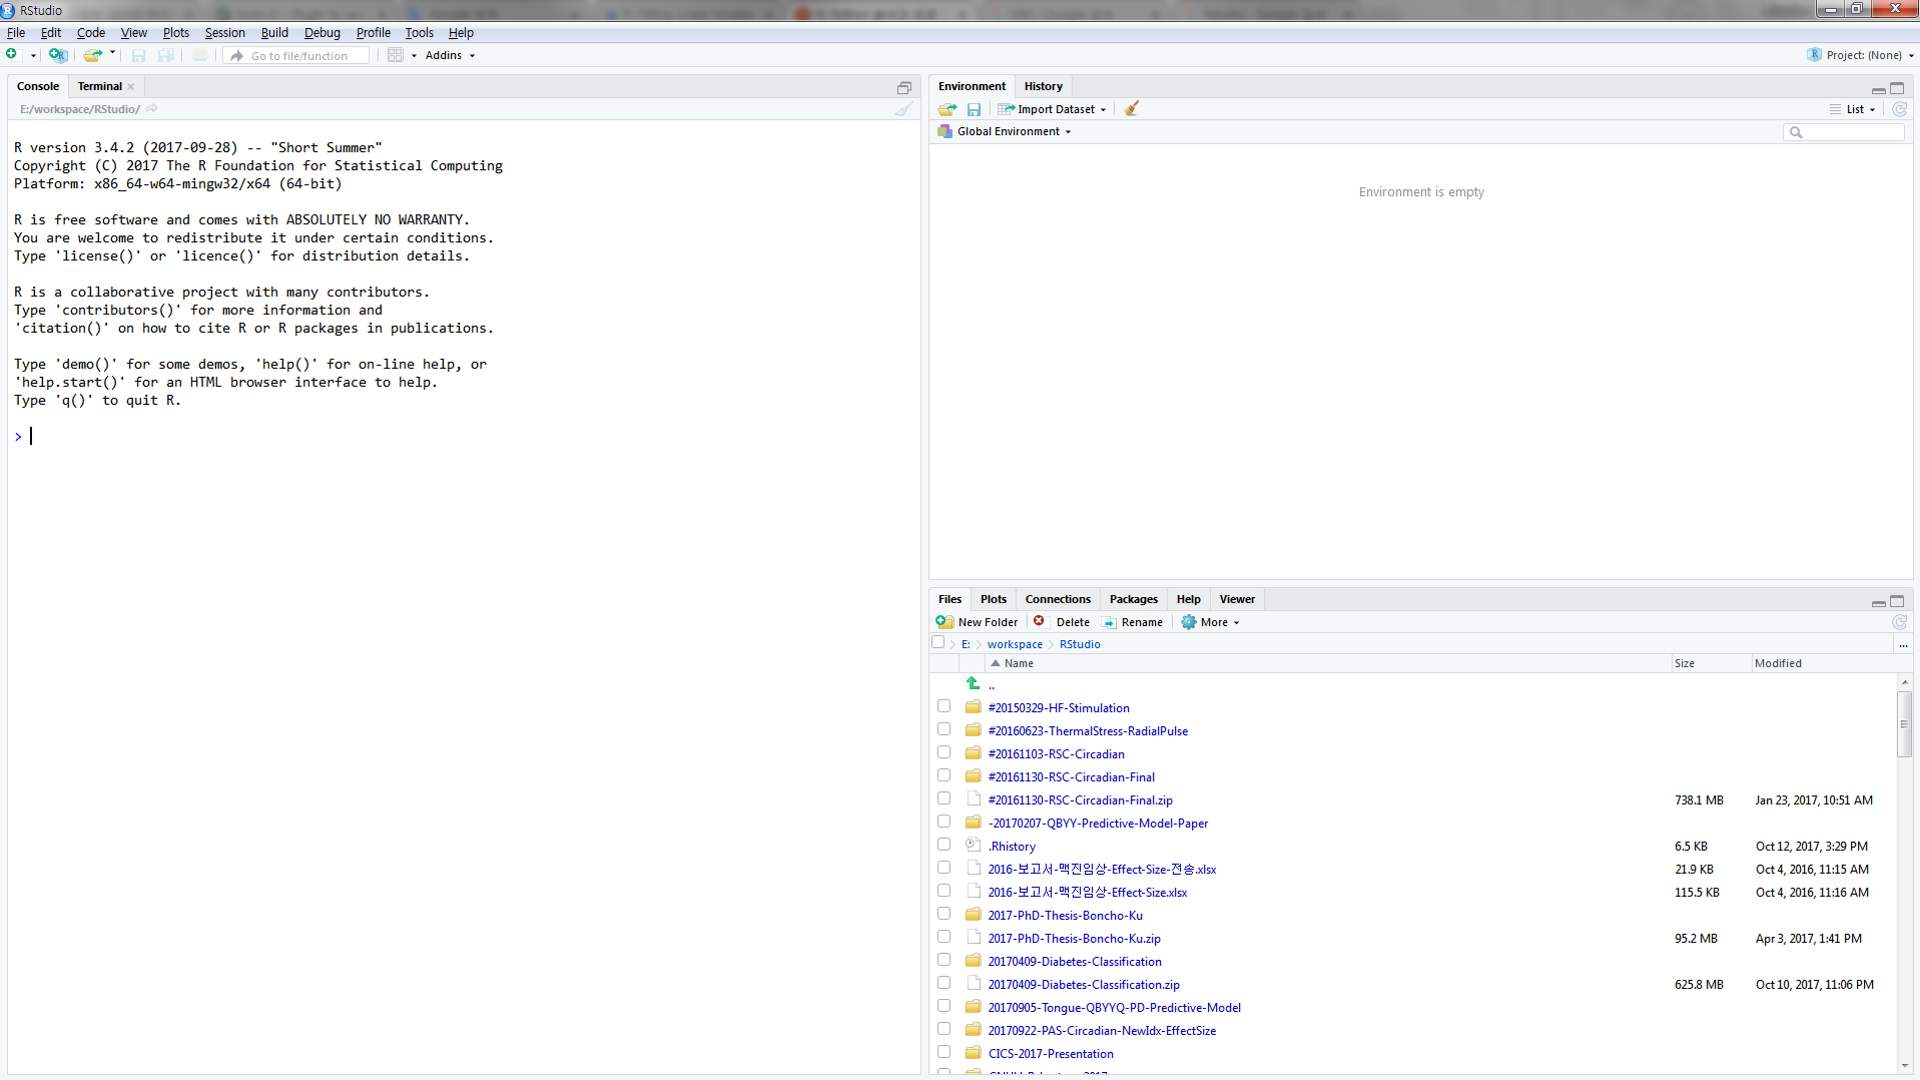
\includegraphics[width=0.8\linewidth]{figures/Rstudio-init} \end{center}

\normalsize

\hypertarget{rstudio-component}{%
\subsection{RStudio IDE 화면 구성}\label{rstudio-component}}

RStudio는 아래 그림과 같이 4개 창으로 구성\footnote{각 창의 위치는 세팅 구성에 따라 달라질 수 있음. 창 구성 방법은 RStudio 환경 옵션 설정에서 설명함.}

\footnotesize

\begin{figure}

{\centering 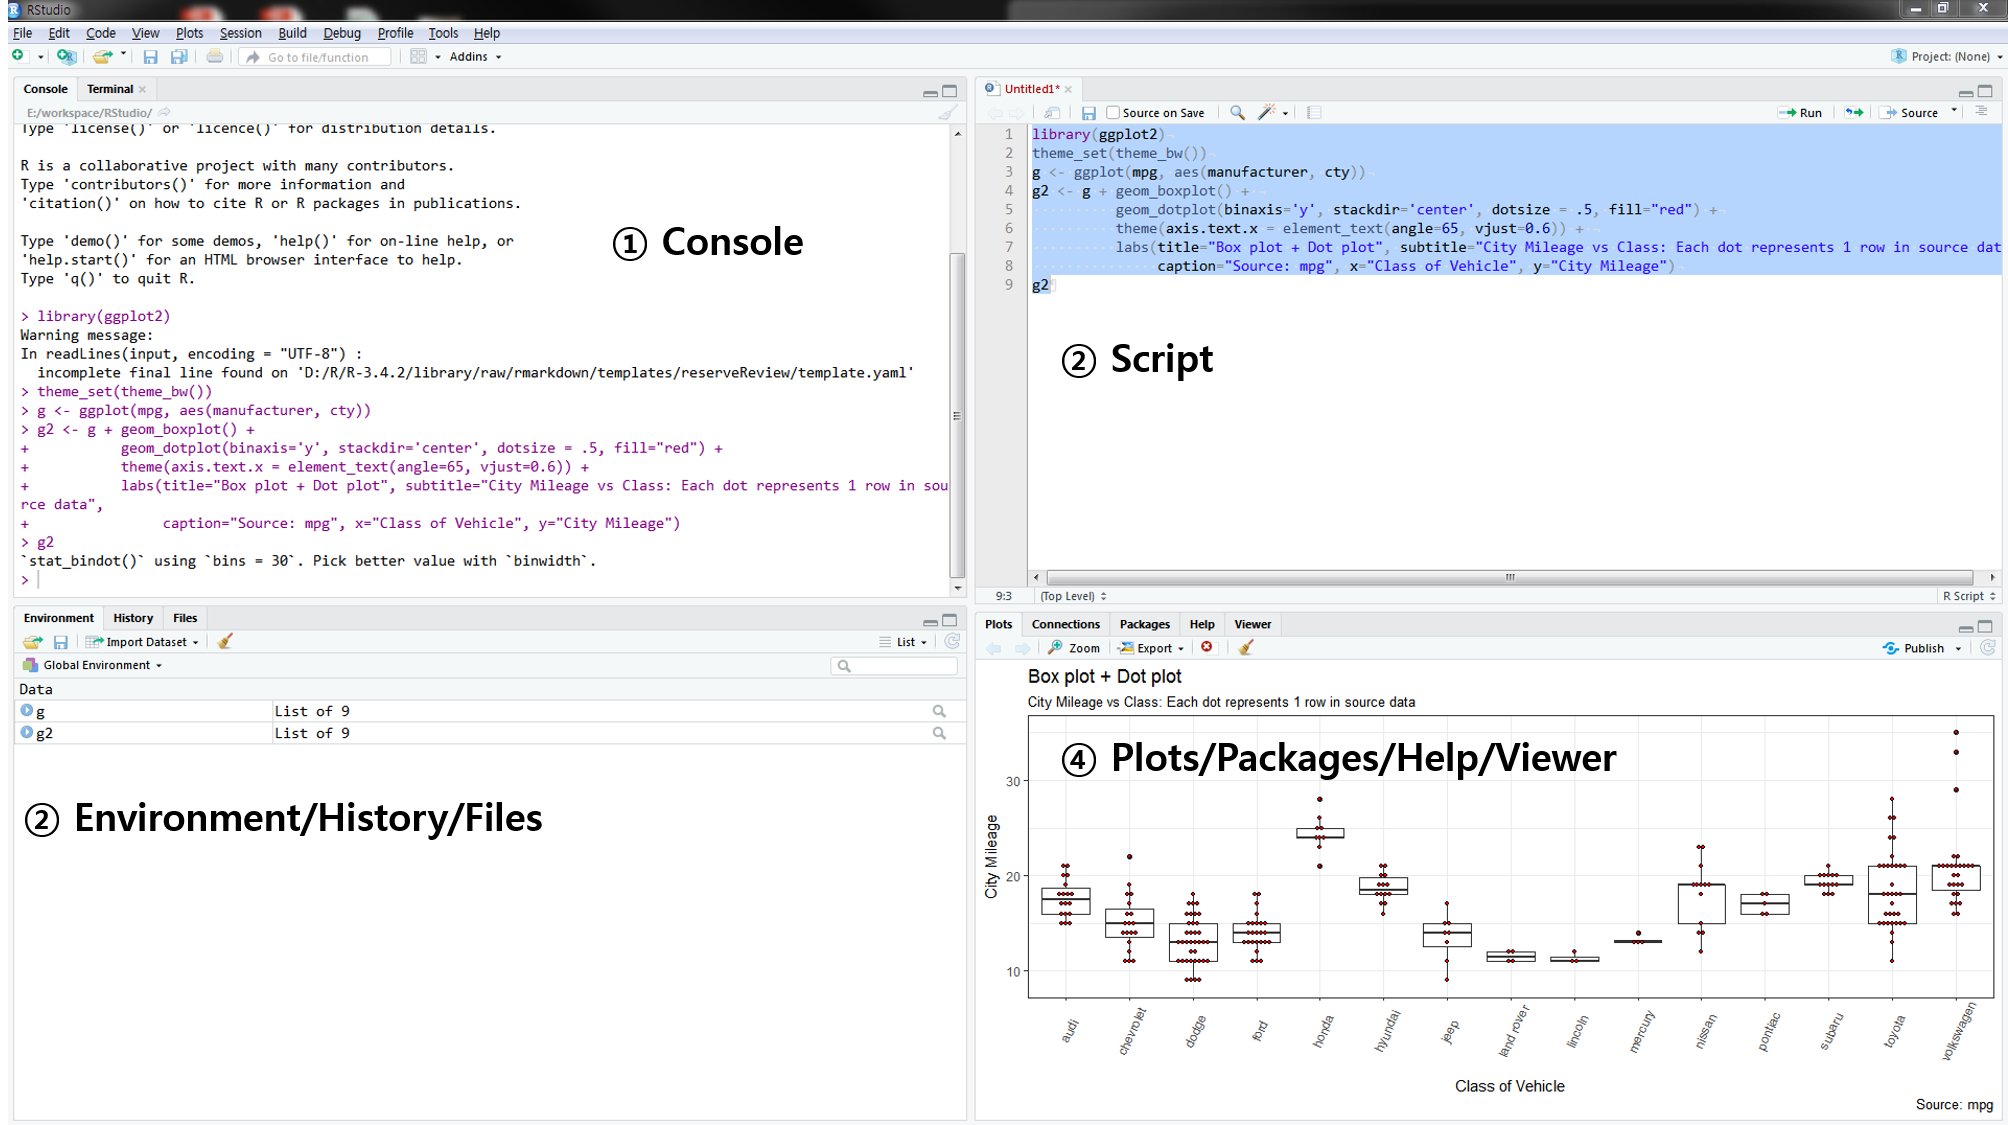
\includegraphics[width=0.9\linewidth]{figures/Rstudio-cap1} 

}

\caption{RStudio 화면구성: 우하단 그림은 http://r-statistics.co/Top50-Ggplot2-Visualizations-MasterList-R-Code.html 에서 발췌}\label{fig:rstudio-windows}
\end{figure}

\normalsize

\textbf{1. 콘솔(console)}

\begin{itemize}
\tightlist
\item
  R 명령어 실행공간(RGui, 정확하게는 R 설치 디렉토리에서 ``\textasciitilde/R/R.x.x/bin/x64/Rterm.exe'' 가 구동되고 있는 공간)
\item
  R script 또는 콘솔 창에서 작성한 명령어(프로그램) 실행 및 그 결과 출력
\item
  경고, 에러/로그 등의 메세지 확인
\end{itemize}

\footnotesize

\begin{figure}

{\centering 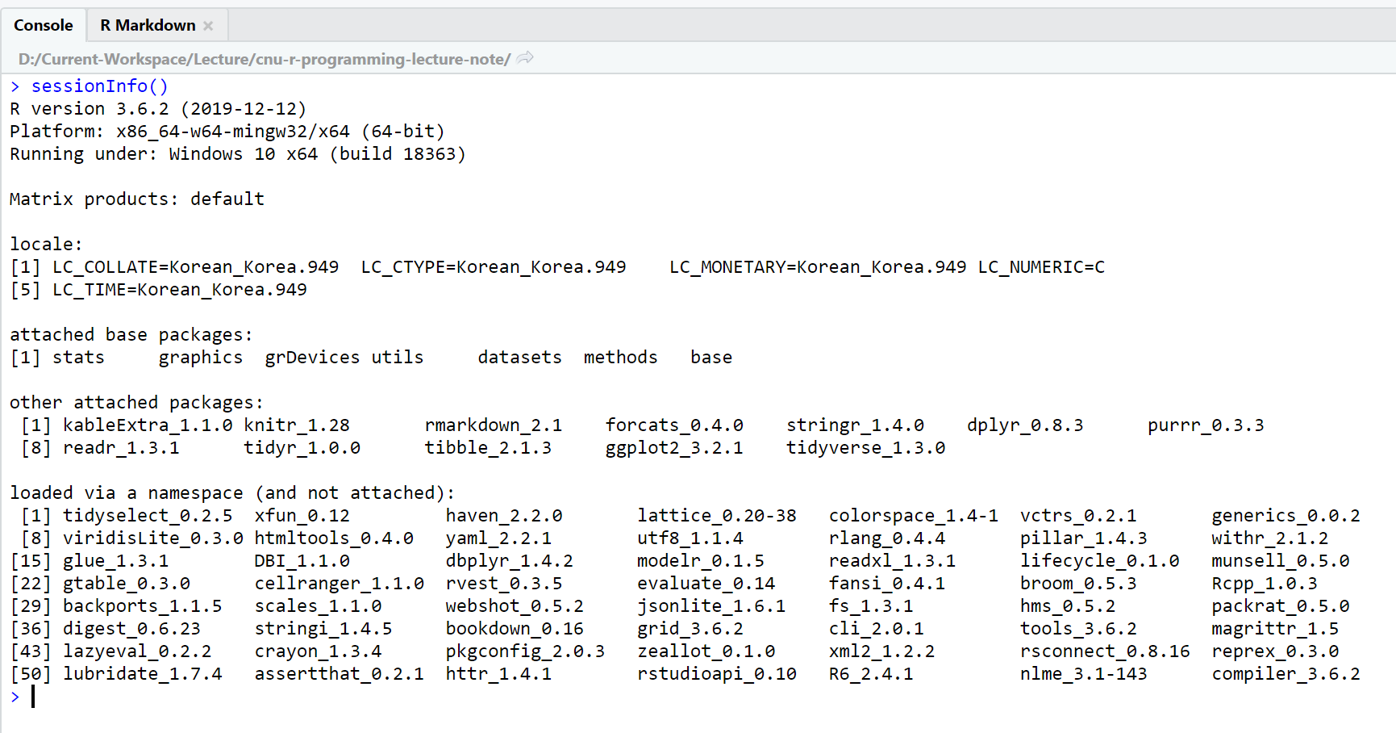
\includegraphics[width=0.8\linewidth]{figures/rstudio-console} 

}

\caption{RStudio 콘솔창에서 명령어 실행 후 출력결과 화면}\label{fig:rstudio-console}
\end{figure}

\normalsize

\textbf{2. 스크립트(script)} (Figure \ref{fig:rstudio-new-script})

\begin{itemize}
\tightlist
\item
  R 명령어 입력 공간으로 일괄처리(batch processing) 가능
\item
  새로운 스크립트 창 열기

  \begin{itemize}
  \tightlist
  \item
    아래 그림과 같이 pull-down 메뉴 좌측 상단 아이콘 클릭 후 {[}R script{]} 선택
  \item
    \texttt{{[}File{]}} \(\rightarrow\) \texttt{{[}New\ File{]}} \(\rightarrow\) \texttt{{[}R\ Script{]}} 선택
  \item
    단축 키: \texttt{{[}Ctrl{]}\ +\ {[}Shift{]}\ +\ {[}N{]}}
  \end{itemize}
\item
  일괄 명령어 처리를 위한 RStudio 제공 단축 키

  \begin{itemize}
  \tightlist
  \item
    \texttt{{[}Ctrl{]}\ +\ {[}Enter{]}}: 선택한 블럭 내 명령어 실행
  \item
    \texttt{{[}Alt{]}\ +\ {[}Enter{]}}: 선택 없이 커서가 위치한 라인의 명령어 실행
  \end{itemize}
\item
  R 스크립트 이외 R Markdown, R Notebook, Shiny web application 등 새 문서의 목적에 따라 다양한 종류의 소스 파일 생성 가능
\item
  저장된 R 스크립트 파일은 \texttt{파일명.R}로 저장됨
\item
  파일 실행 방법

  \begin{itemize}
  \tightlist
  \item
    실행하고자 하는 파일을 읽은 후(\texttt{{[}File{]}} \(\rightarrow\) \texttt{{[}Open\ File{]}} + 파일명 선택 또는 \texttt{파일명.R} 더블 클릭) 입력된 모든 라인을 선택한 뒤 \texttt{{[}Ctrl{]}\ +\ {[}Enter{]}}
  \item
    파일 읽은 후 \texttt{{[}Ctrl{]}\ +\ {[}Shift{]}\ +\ {[}S{]}} (현재 열려있는 \texttt{*.R} 파일에 대해) 또는 \texttt{{[}Ctrl{]}\ +\ {[}Shift{]}\ +\ {[}Enter{]}}
  \end{itemize}
\end{itemize}

\footnotesize

\begin{figure}

{\centering 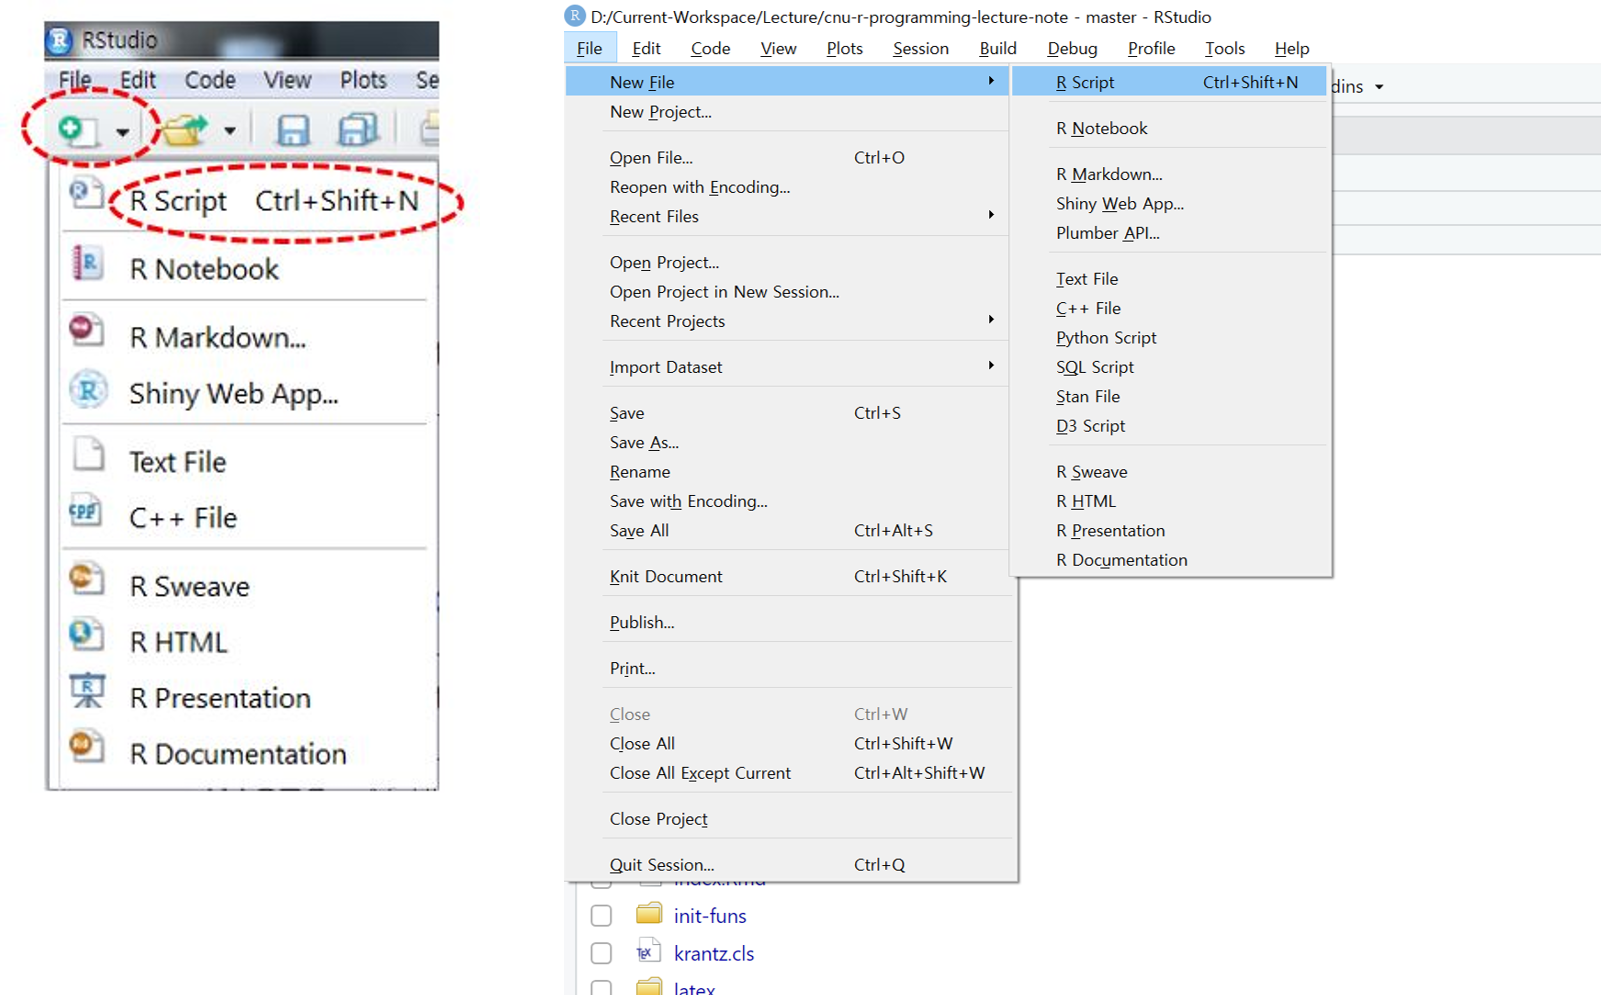
\includegraphics[width=0.8\linewidth]{figures/rstudio-open-new-script} 

}

\caption{RStudio 스크립트 새로 열기}\label{fig:rstudio-new-script}
\end{figure}

\normalsize

\footnotesize

\BeginKnitrBlock{rmdtip}
RStudio는 코딩 및 소스 작성의 효율성을 위해 여러 가지 단축 키를 제공하고 있음. 단축키는 아래 그림과 같이 pull down 메뉴 \texttt{{[}Tools{]}} 또는 \texttt{{[}Help{]}}에서 \texttt{{[}Keyboard\ shortcut\ help{]}} 또는 \texttt{{[}Alt{]}\ +\ {[}Shift{]}\ +\ {[}K{]}} 단축키를 통해 확인할 수 있음. 또는 Rstudio cheatsheet에서 단축키에 대한 정보를 제공하는데 pull down 메뉴 \texttt{{[}Help{]}} \(\rightarrow\) \texttt{{[}Cheatsheets{]}} \(\rightarrow\) \texttt{{[}RStudio\ IDE\ Cheat\ Sheet{]}}을 선택하면 각 아이콘 및 메뉴 기능에 대한 개괄적 설명 확인 가능함.
\EndKnitrBlock{rmdtip}

\normalsize

\textbf{3. 환경/명령기록(Environment/History)} (Figure \ref{fig:rstudio-env})

\begin{itemize}
\tightlist
\item
  \textbf{Environment}: 현재 R 작업환경에 저장되어 있는 객체의 특성 및 값 등을 요약 제시

  \begin{itemize}
  \tightlist
  \item
    좌측 아래 화살표 버튼 클릭: 해당 객체의 상세 정보 확인
  \item
    우측 사각형 버튼 또는 객체(데이터셋명) 클릭: 객체가 데이터셋(데이터프레임)인 경우 스프레드 시트 형태로 데이터셋 확인
  \end{itemize}
\end{itemize}

\footnotesize

\begin{figure}

{\centering 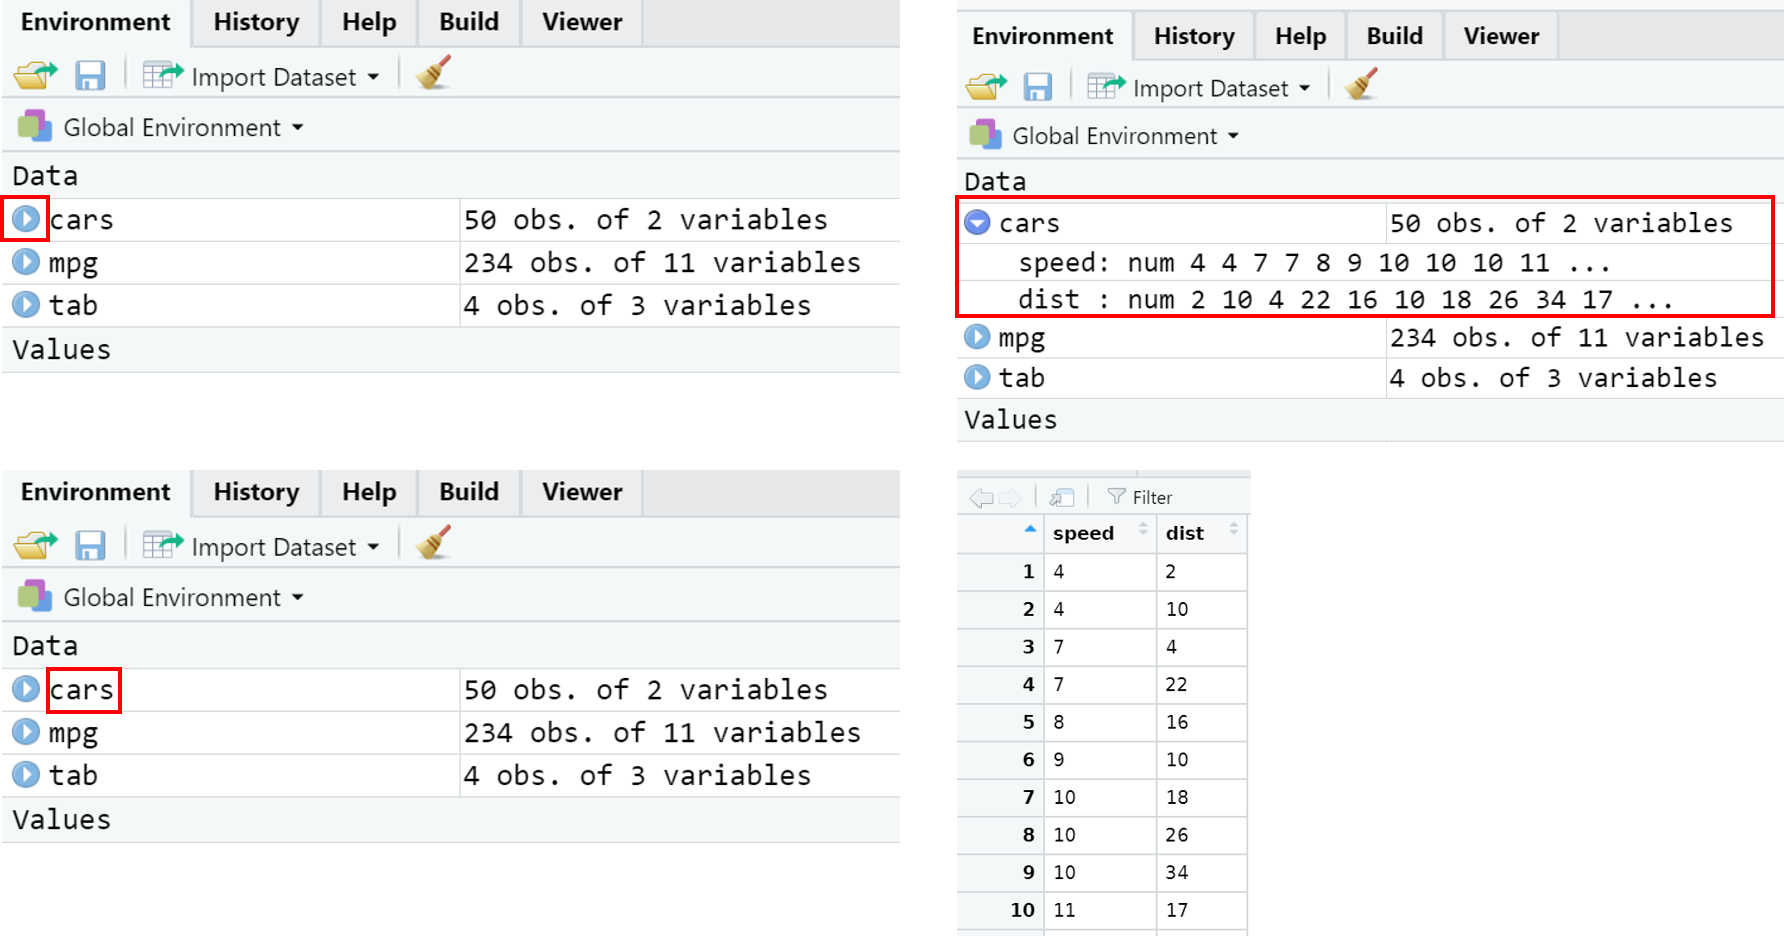
\includegraphics[width=0.9\linewidth]{figures/rstudio-environment} 

}

\caption{RStudio Environment 창 객체 상세 정보 및 스프레드 시트 출력 결과}\label{fig:rstudio-env}
\end{figure}

\normalsize

\begin{itemize}
\tightlist
\item
  History: R 콘솔에서 실행된 명령어(스크립트)들의 이력 확인
\end{itemize}

\footnotesize

\begin{center}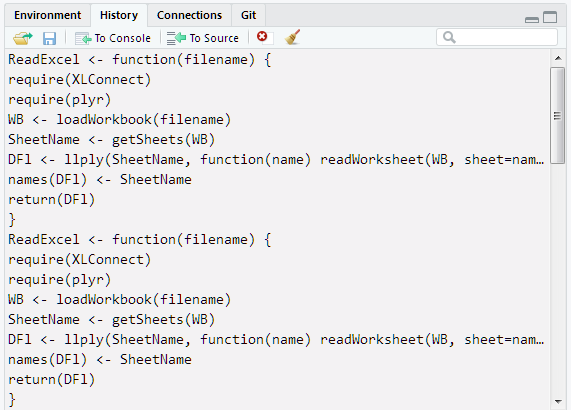
\includegraphics[width=0.9\linewidth]{figures/Rstudio-historywin} \end{center}

\normalsize

\textbf{4. File/Plots/Packages/Help/Viewer}

\begin{itemize}
\tightlist
\item
  File: Windows 파일 탐색기와 유사한 기능 제공

  \begin{itemize}
  \tightlist
  \item
    파일 및 폴더 생성, 삭제/파일 및 폴더명 수정, 그리고 작업경로 설정
  \end{itemize}
\end{itemize}

\footnotesize

\begin{center}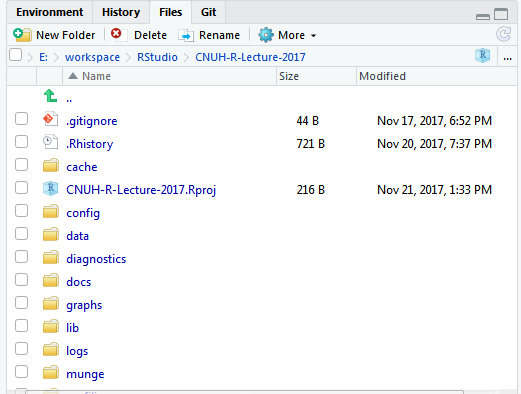
\includegraphics[width=0.8\linewidth]{figures/Rstudio-file} \end{center}

\normalsize

\begin{itemize}
\tightlist
\item
  \textbf{Plots}: 생성한 그래프 출력

  \begin{itemize}
  \tightlist
  \item
    작업 중 생성한 그래프 이력이 Plots 창에 저장: \(\leftarrow\) 이전, \(\rightarrow\) 최근
  \item
    \textbf{\texttt{Zoom}}: 클릭 시 해당 그래프의 팝업창이 생성되고 팝업창의 크기 조정을 통해 그래프의 축소/확대 가능
  \item
    \textbf{\texttt{Export}}: 선택한 그래프를 이미지 파일(\texttt{.png}, \texttt{.jpeg}, \texttt{.pdf} 등)로 저장할 수 있고, 클립보드로 복사 가능
  \end{itemize}
\end{itemize}

\footnotesize

\begin{center}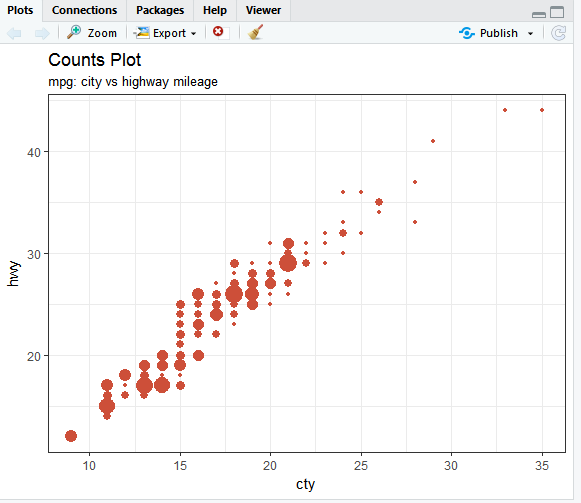
\includegraphics[width=0.8\linewidth]{figures/RStudio-plotwin} \end{center}

\normalsize

\begin{itemize}
\tightlist
\item
  \textbf{Packages}: 현재 컴퓨터에 설치된 R 패키지 목록 출력

  \begin{itemize}
  \tightlist
  \item
    신규 설치 및 업데이트 가능
  \end{itemize}
\end{itemize}

\footnotesize

\begin{center}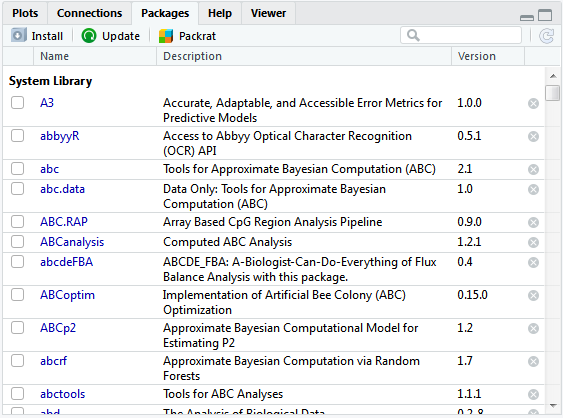
\includegraphics[width=0.8\linewidth]{figures/RStudio-packagewin} \end{center}

\normalsize

\begin{itemize}
\tightlist
\item
  \textbf{Help}: \texttt{help(topic)} 입력 시 도움말 창이 출력되는 공간
\end{itemize}

\footnotesize

\begin{Shaded}
\begin{Highlighting}[]
\KeywordTok{help}\NormalTok{(lm)}
\end{Highlighting}
\end{Shaded}

\normalsize

\footnotesize

\begin{center}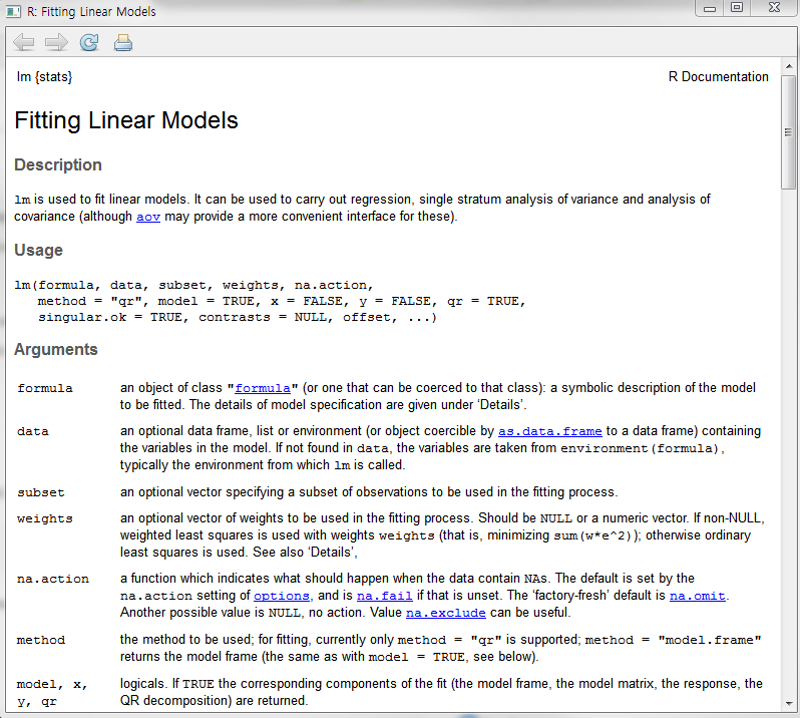
\includegraphics[width=0.8\linewidth]{figures/RStudio-helpwin} \end{center}

\normalsize

\hypertarget{rstudio-glob-options}{%
\subsection{RStudio 환경 설정}\label{rstudio-glob-options}}

Pull-down 메뉴에서 \texttt{{[}Tools{]}} \(\rightarrow\) \texttt{{[}Global\ Options...{]}}를 선택

\footnotesize

\begin{center}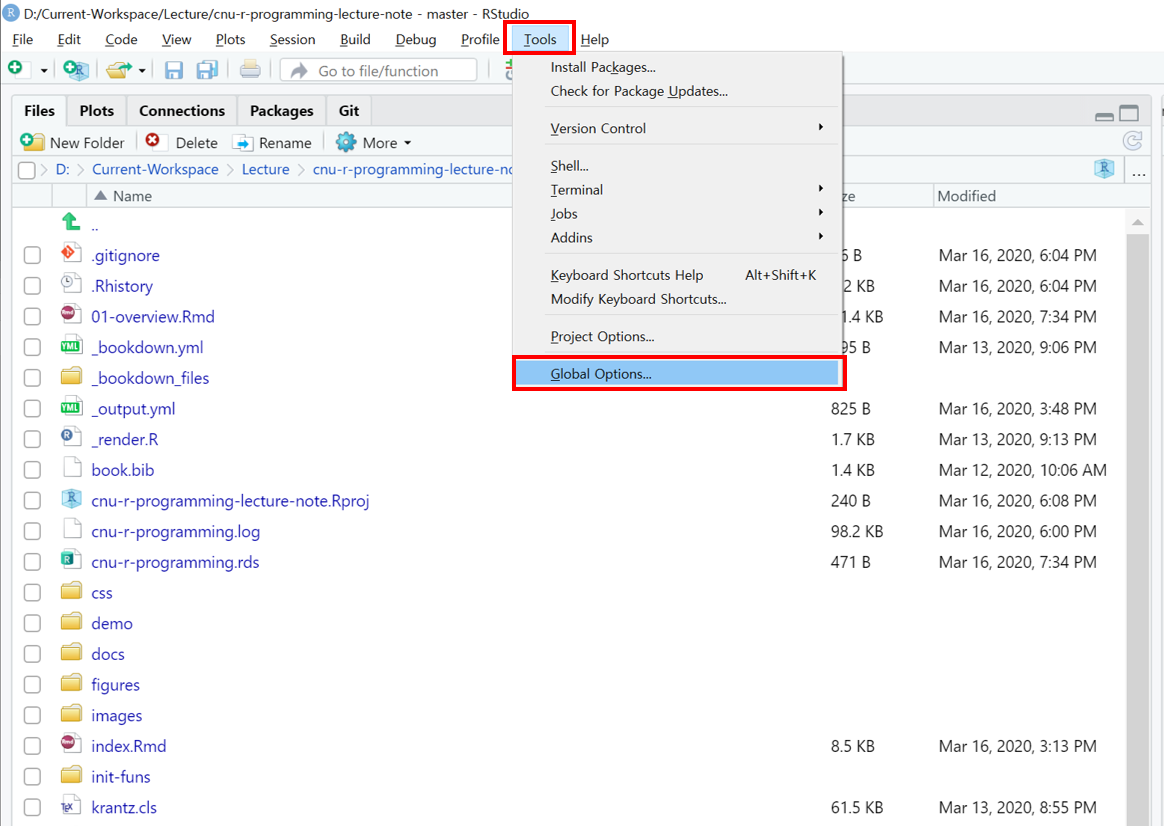
\includegraphics[width=0.8\linewidth]{figures/rstudio-glob-menu} \end{center}

\normalsize

\textbf{General}: RStudio 운용 관련 전반적 설정 세팅

\footnotesize

\begin{center}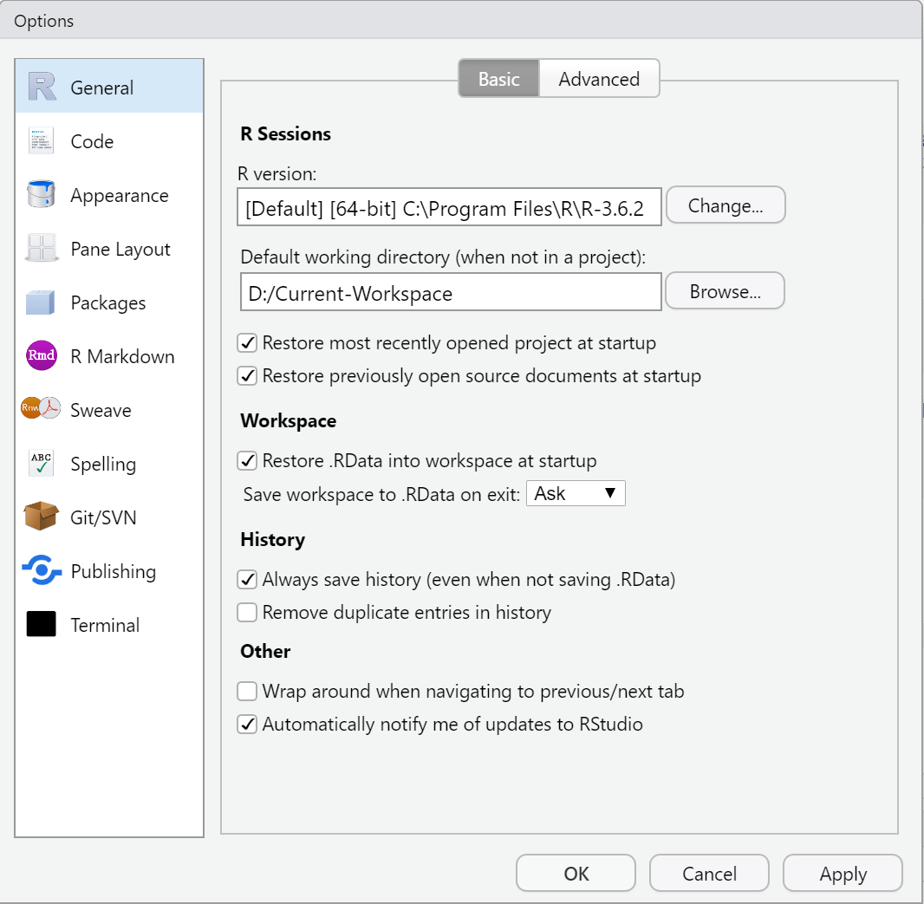
\includegraphics[width=0.8\linewidth]{figures/rstudio-glob-option} \end{center}

\normalsize

\begin{itemize}
\tightlist
\item
  \textbf{R version}: 만약 컴퓨터에 두 개 이상 다른 R 버전이 설치되어 있는 경우 \texttt{{[}Change{]}} 클릭 후 설정 변경 가능
\item
  \textbf{Default Working directory}: 작업 디렉토리 지정({[}\texttt{Browse}{]} 클릭 후 임의 폴더 설정 가능)
\item
  \textbf{Restore most recently opened project at startup}: RStudio 실행 시 가장 최근에 작업한 프로젝트로 이동
\item
  \textbf{Restore previously open source documents at startup}: RStudio 실행 시 현재 프로젝트에서 가장 최근에 작업한 소스코드 문서를 함께 열어줌.
\item
  \textbf{Restore .RData into workspace at startup}: 작업 디렉토리에 존재하는 \texttt{.RData} 파일을 RStudio 실행 시 불러옴
\item
  \textbf{Save workspace to .RData on exit}: R workspace 자동 저장(\texttt{.RData}) 여부
\item
  \textbf{Always save history (even when not saving .RData) }: R 실행 명령 history 저장 여부(Always/Never/Ask)
\item
  \textbf{Remove duplicate entries in history}: history 저장 시 중복 명령 제거 여부
\end{itemize}

\textbf{Code: Editing}: 들여쓰기, 자동 줄바꿈 등 코드 편집에 대한 전반적 설정

\footnotesize

\begin{center}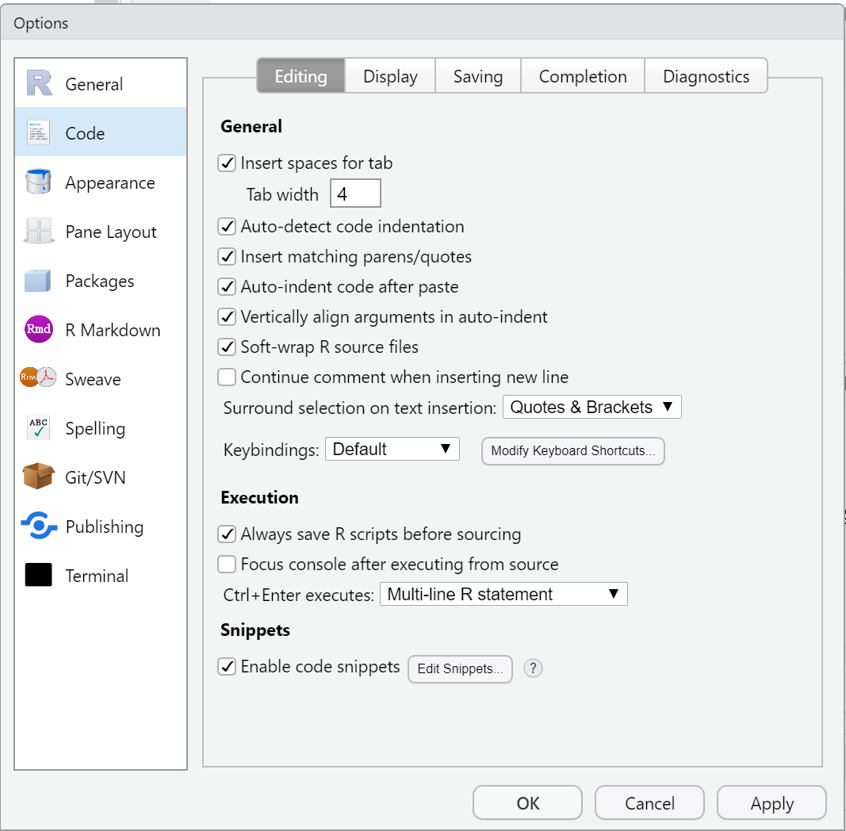
\includegraphics[width=0.8\linewidth]{figures/rstudio-code-edit-option} \end{center}

\normalsize

\begin{itemize}
\tightlist
\item
  \textbf{Insert spaces for tab}: \texttt{{[}Tab{]}} 키를 눌렀을 때 공백(space) 개수 결정(본 강의노트: \texttt{Tab\ width\ =\ 4})
\item
  \textbf{Auto-detect code indentation}: 코들 들여쓰기 자동 감지
\item
  \textbf{Insert matching parens/quotes}: 따옴표, 괄호 입력 시 커서를 따옴표/괄호 사이로 자동 이동
\item
  \textbf{Auto-indent code after paste}: 코드 복사 시 들여쓰기 일괄 적용
\item
  \textbf{Vertically align arguments in auto-indent}: 함수 작성 시 들여쓰기 레벨 유지 여부
\item
  \textbf{Soft-wrap R source file}: 스크립트 편집기 너비를 초과하는 경우 R 코드 행을 자동 줄바꿈
\item
  \textbf{Continue comment when inserting new line}: 주석 표시를 다음 행에도 자동 적용 여부
\item
  \textbf{Surround selection on text insertino}: 스크립트 상 text 선택 후 자동 따옴표 및 괄호 적용 여부
\item
  \textbf{Focus console after executing from source}: 스크립트 실행 후 커서 위치를 콘솔로 이동 여부
\end{itemize}

\textbf{Code: Display}: 스크립트(소스) 에디터 표시 화면 설정

\footnotesize

\begin{center}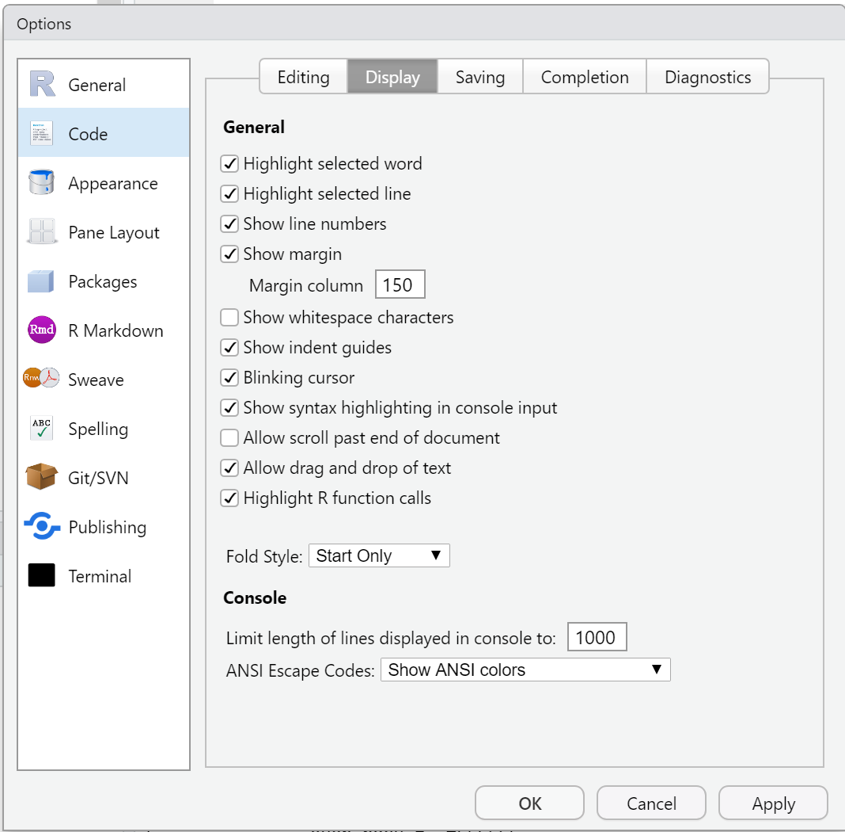
\includegraphics[width=0.8\linewidth]{figures/rstudio-code-display} \end{center}

\normalsize

\begin{itemize}
\tightlist
\item
  \textbf{Highlight selected word}: 스크립트 내 text 선택 시 동일한 text에 대해 배경강조 효과 여부
\item
  \textbf{Highlight selected line}: 선택된 행에 대해 배경 강조효과 여부
\item
  \textbf{Show line numbers}: 행 번호 보여주기 여부
\item
  \textbf{Show margin}: 소스 에디터 오른 쪽에 지정한 margin column 보여주기 여부
\item
  \textbf{Show whitespace characters}: 에디터에 공백 표시 여부
\item
  \textbf{Show indent guides}: 현재 들여쓰기 열 표시 여부
\item
  \textbf{Blinking cursor}: 커서 깜박임 여부
\item
  \textbf{Show syntax highlighting in console output}: 콘솔 입력 라인에 R 구문 강조 표시 적용 여부
\item
  \textbf{Allow scroll past end of document}: 문서 마지막 행 이후 스크롤 허용 여부
\item
  \textbf{Allow drag and drop of text}: 선택한 복수의 행으로 구성된 text에 대해 마우스 drag 허용
\item
  \textbf{Highlight R function calls}: R 내장 및 패키지 제공함수에 대해 강조 여부
\end{itemize}

\textbf{Code: Saving}: 스크립트(소스) 에디터 저장 설정

\footnotesize

\begin{center}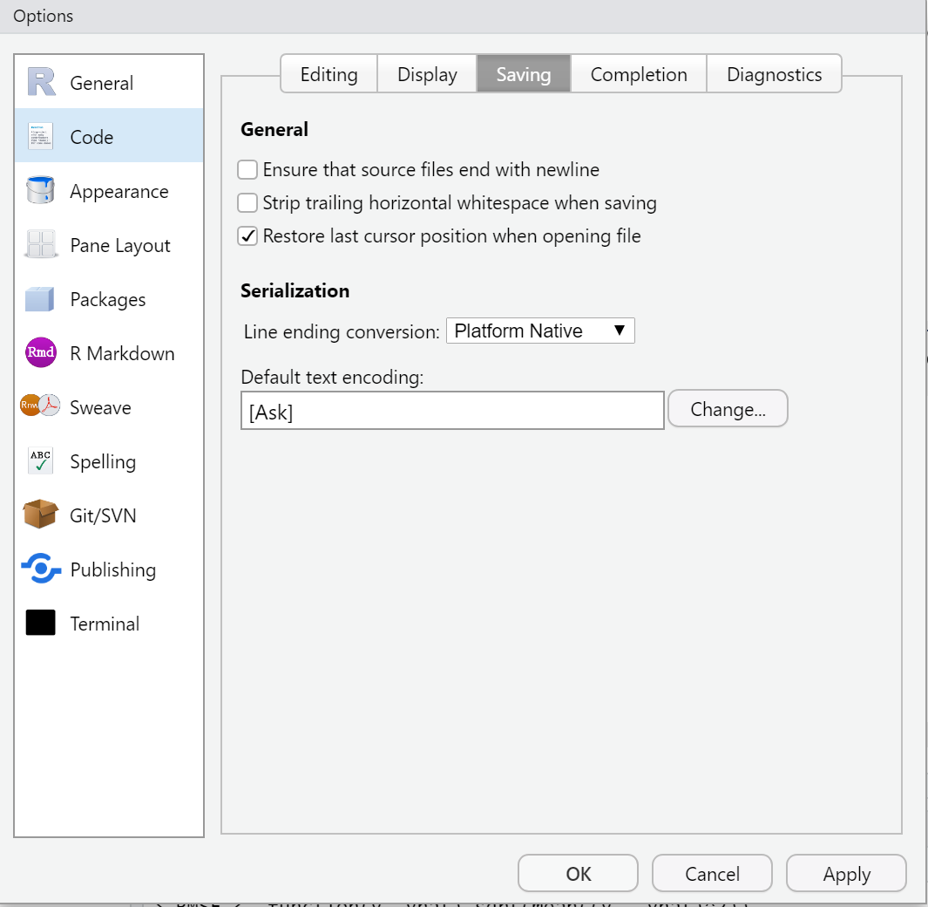
\includegraphics[width=0.8\linewidth]{figures/rstudio-code-saving} \end{center}

\normalsize

\begin{itemize}
\tightlist
\item
  \textbf{Ensure that source file end with newline}:
\item
  \textbf{String trailing horizontal whitespace when saving}:
\item
  \textbf{Restore last cursor position when opening file}:
\item
  \textbf{Default text encoding}:
\end{itemize}

\textbf{Appearance}: RStudio 전체 폰트, 폰트 크기, theme 설정

\footnotesize

\begin{center}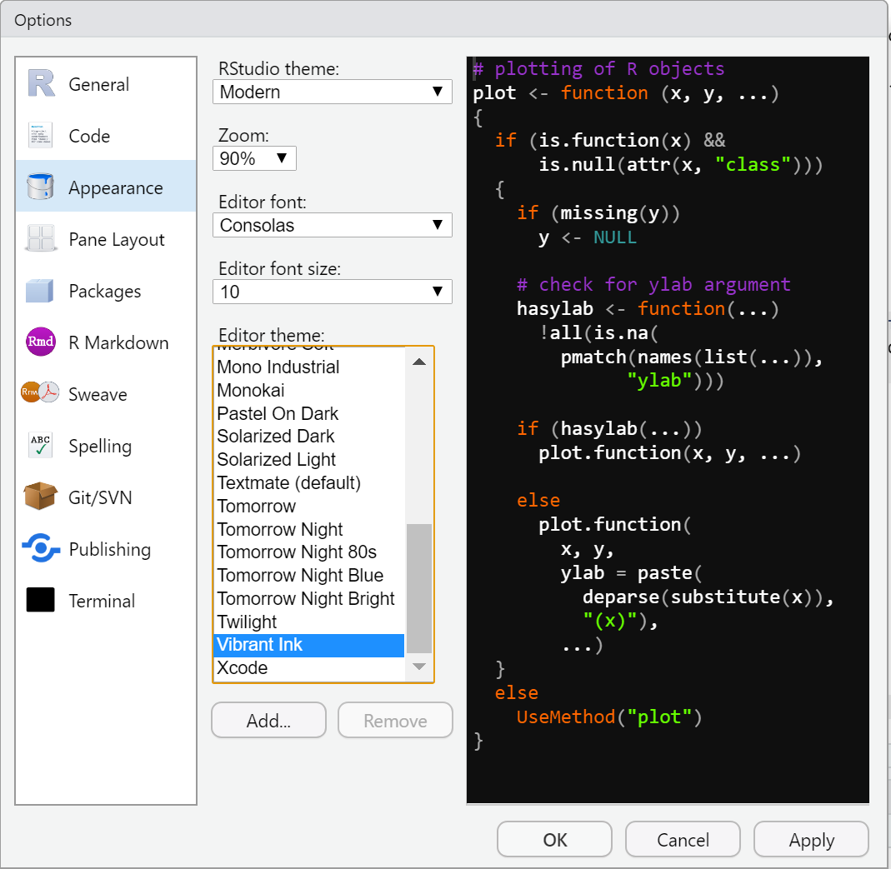
\includegraphics[width=0.8\linewidth]{figures/rstudio-appearance} \end{center}

\normalsize

\textbf{Pane Layout}: RStudio 구성 패널들의 위치 및 항목 등을 수정/추가/삭제(4개 페널은 항시 유지)

\footnotesize

\begin{center}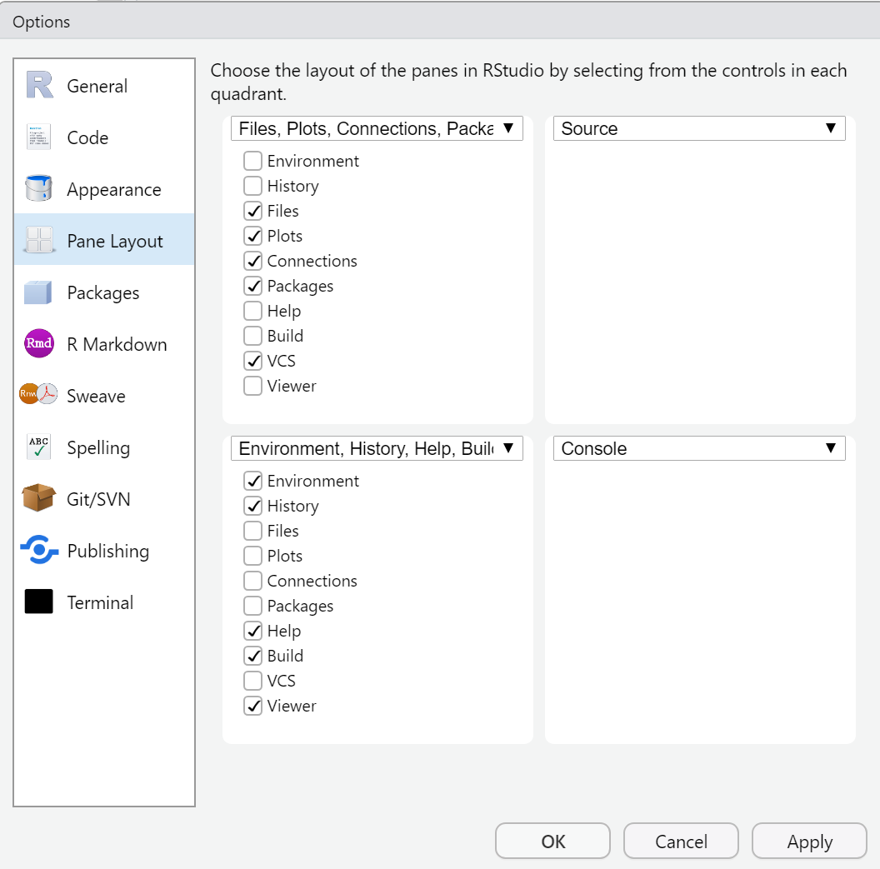
\includegraphics[width=0.8\linewidth]{figures/rstudio-pane-layout} \end{center}

\normalsize

\hypertarget{r-package-installation}{%
\section{R 주요 패키지 설치}\label{r-package-installation}}

\begin{enumerate}
\def\labelenumi{\arabic{enumi}.}
\tightlist
\item
  RStudio 메뉴 \texttt{{[}Tools{]}} \(\rightarrow\) \texttt{{[}Install\ packages{]}} 클릭 후 생성된 팝업 창에서 설치하고자 하는 패키지 입력 후 설치
\item
  RStudio \texttt{Packages} 창에서 \texttt{{[}Install{]}} 버튼 누르고 설치(위와 동일)
\item
  R 콘솔 또는 스크립트 창에서 \texttt{install.packages()} 함수를 사용해서 패키지 설치
\end{enumerate}

\hypertarget{r-package-path}{%
\subsection{R 패키기 Path 지정}\label{r-package-path}}

\hypertarget{r-package-load}{%
\subsection{R 패키지 불러오기}\label{r-package-load}}

\begin{enumerate}
\def\labelenumi{\arabic{enumi}.}
\tightlist
\item
  \texttt{library()} vs.~\texttt{require()}

  \begin{itemize}
  \tightlist
  \item
    \texttt{library()}: 불러오고자 하는 패키지가 시스템에 존재하지 않는 경우 에러 메세지 출력(에러 이후 명령어들이 실행되지 않음)
  \item
    \texttt{require()}: 패키지가 시스템에 존재하지 않는 경우 경고 메세지 출력(경고 이후 명령어 정상적으로 실행)
  \end{itemize}
\item
  다중 패키지 동시에 불러오기

  \begin{itemize}
  \tightlist
  \item
    RStudio \texttt{Packages} 창에서 설치하고자 하는 패키지 선택 버튼 클릭하면 R workspace로 해당 패키지 로드 가능
  \item
    스크립트 이용
  \end{itemize}
\end{enumerate}

\footnotesize

\begin{Shaded}
\begin{Highlighting}[]
\NormalTok{pkgName <-}\StringTok{ }\KeywordTok{c}\NormalTok{(}\StringTok{"MASS"}\NormalTok{, }\StringTok{"tidyverse"}\NormalTok{, }\StringTok{"ggthemes"}\NormalTok{, }\StringTok{"readxl"}\NormalTok{, }
             \StringTok{"kableExtra"}\NormalTok{, }\StringTok{"ztable"}\NormalTok{, }\StringTok{"car"}\NormalTok{, }\StringTok{"lsmeans"}\NormalTok{, }
             \StringTok{"rmarkdown"}\NormalTok{, }\StringTok{"knitr"}\NormalTok{)}
\CommentTok{# 'lapply()': 벡터, 리스트 또는 표현식에 함수를 적용하여 그 결과를 리스트로 반환}
\KeywordTok{lapply}\NormalTok{(pkgName, require, }\DataTypeTok{character.only =}\NormalTok{ T) }
\end{Highlighting}
\end{Shaded}

\normalsize

\hypertarget{rstudio-create-project}{%
\section{RStudio 프로젝트 생성}\label{rstudio-create-project}}

\hypertarget{rstudio-project}{%
\subsection{RStudio 프로젝트}\label{rstudio-project}}

\begin{enumerate}
\def\labelenumi{\arabic{enumi}.}
\tightlist
\item
  프로젝트

  \begin{itemize}
  \tightlist
  \item
    물리적 측면: 최종 산출물(문서)를 생성하기 위한 데이터, 사진, 그림 등을 모아 놓은 폴더
  \item
    논리적 측면: R 세션 및 작업의 버전 관리
  \end{itemize}
\item
  프로젝트의 필요성

  \begin{itemize}
  \tightlist
  \item
    자료의 정합성 보장
  \item
    다양한 확장자를 갖는 한 폴더 내에 뒤섞일 때 곤란해 질 수 있음
  \item
    실제 분석 및 그래프 생성에 사용한 정확한 프로그램 또는 코드 연결이 어려움
  \end{itemize}
\item
  좋은 프로젝트 구성을 위한 방법

  \begin{itemize}
  \tightlist
  \item
    원자료(raw data)의 보호: 가급적 자료를 읽기 전용(read only) 형태로 다루기
  \item
    데이터 정제(data wrangling 또는 data munging)를 위한 스크립트와 정제 자료를 보관하는 읽기 전용 데이터 디렉토리 생성
  \item
    작성한 스크립트로 생성한 모든 산출물(테이블, 그래프 등)을 ``일회용품''처럼 처리 \(\rightarrow\) 스크립트로 재현 가능
  \item
    한 프로젝트 내 각기 다른 분석마다 다른 하위 디렉토리에 출력결과 저장하는 것이 유용
  \end{itemize}
\item
  RStudio 새로운 프로젝트 생성

  \begin{itemize}
  \tightlist
  \item
    RStudio의 가장 강력하고 유용한 기능
  \item
    새로운 프로젝트 생성: RStudio 메뉴에서 \texttt{{[}File{]}} \(\rightarrow\) \texttt{{[}New\ Project{]}} 선택하면 아래와 같은 팝업 메뉴 생성
  \end{itemize}
\end{enumerate}

\hypertarget{r-markdown-get-start}{%
\section{R Markdown (맛보기)}\label{r-markdown-get-start}}

  \bibliography{book.bib,packages.bib}

\printindex

\end{document}
